\chapter{Laboratorio 3}
\noindent Per le simulazioni condotte in questo laboratorio è stato impiegato il medesimo strumento software del Laboratorio 2 (\texttt{Laser.m}). Tuttavia, l'oggetto
dell'analisi è ora un diodo laser a monomodo ottico (modello a singola popolazione \textit{bulk}). Pertanto, i parametri geometrici della cavità e i parametri del materiale
sono stati impostati sui valori specifici forniti per la struttura laser in esame. Come richiesto dalla procedura di simulazione, l'analisi statica è stata eseguita
preventivamente per ricavare il punto di lavoro permanente e le condizioni di soglia, i cui risultati costituiscono l'input fondamentale per le successive analisi dinamiche.

\section{Caratteristica statica di un diodo laser a singolo modo}
\noindent Mediante l'opzione \textit{Static Analysis} del simulatore, impostando la lunghezza d'onda di lavoro a $\lambda = 1550\text{ nm}$ e gli opportuni parametri fisici
e geometrici, sono state ricavate le caratteristiche statiche del diodo laser in funzione della corrente d'ingresso $I$.\\ Si precisa che il simulatore utilizza un modello
di guadagno lineare del tipo:
\[ 
g(N) = a_0(N - N_{\text{tr}})
\] 
dove $g(N)$ è il guadagno ottico in funzione dei portatori, $a_0$ è il coefficiente di guadagno differenziale e $N_{tr}$ è la densità di portatori alla trasparenza (ossia quando
il guadagno è nullo).

\noindent\\ In Figura \ref{fig:P_N_Lw_vs_I_ah1} sono riportati gli andamenti della potenza ottica in uscita $P_{\text{out}}$, della densità di portatori $N$ e della
larghezza di riga spettrale (\textit{optical linewidth}) $\Delta\nu$ al variare di $I$.
\\ Si precisa che, in questa prima analisi, è stato impostato un valore del \textit{Linewidth Enhancement Factor (LEF)} pari a $\boldsymbol{\alpha_H = 1}$.

\begin{figure}[!h]
 \centering
 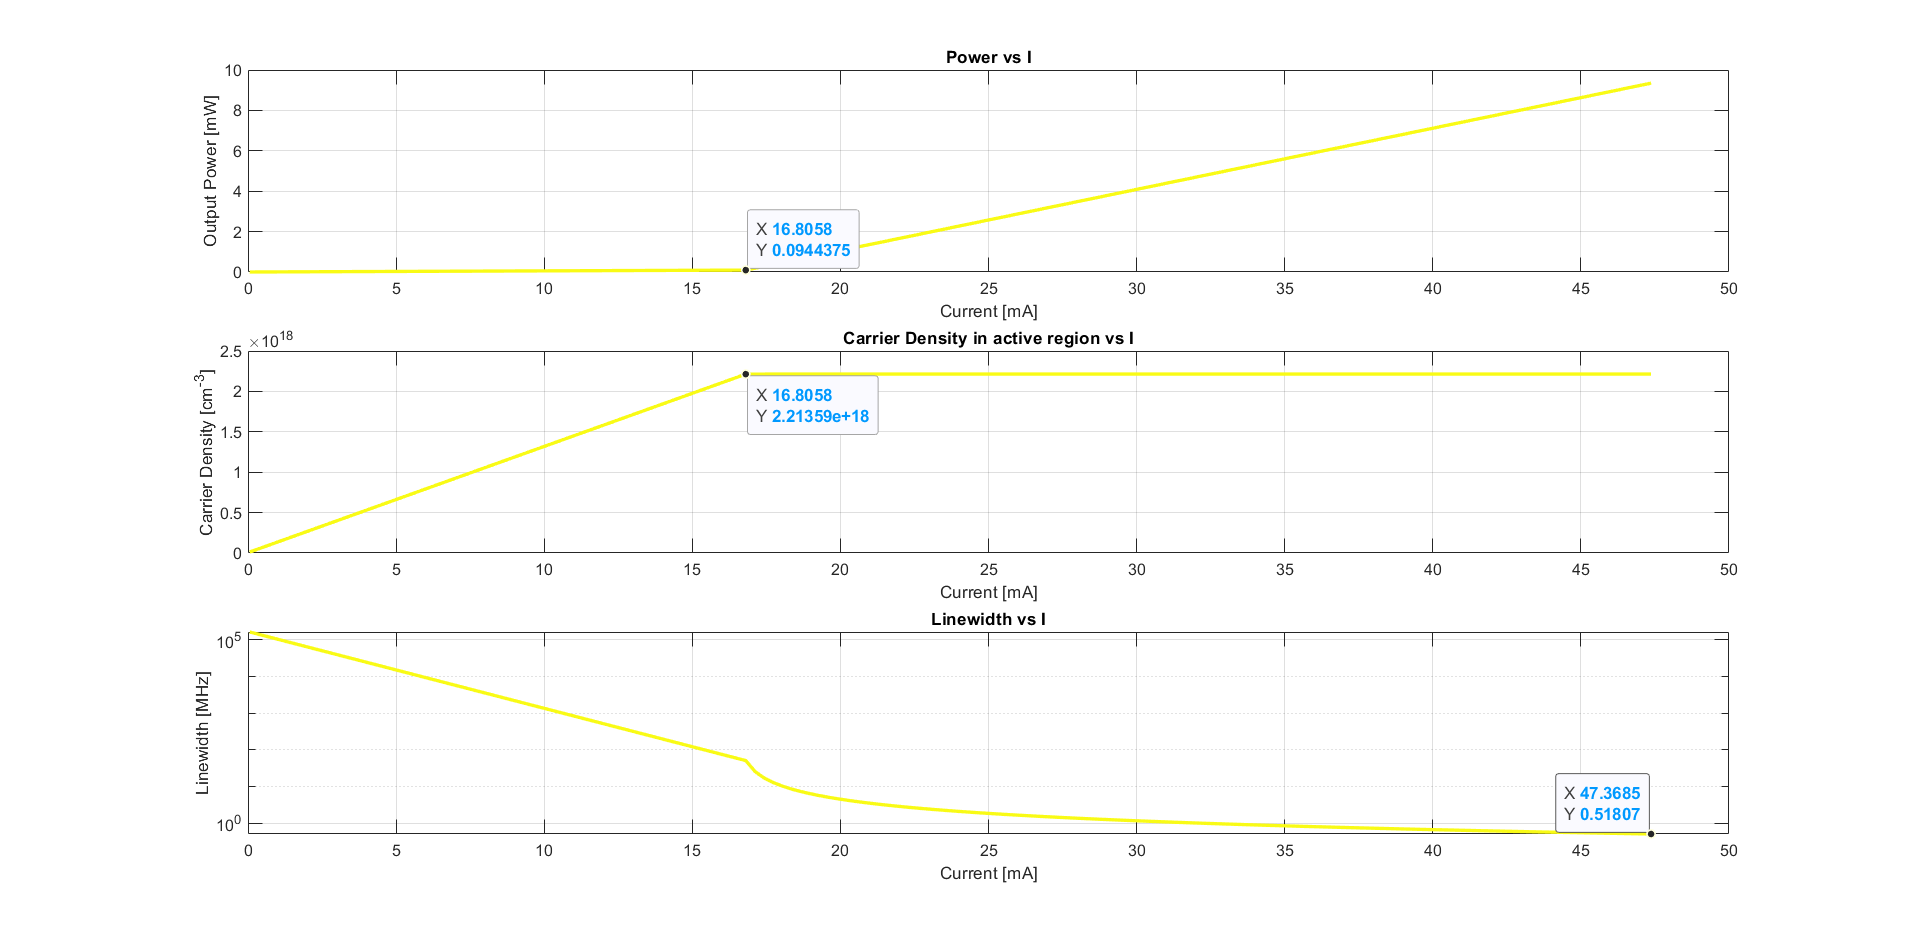
\includegraphics[width=14cm]{lab3/Images/prob1/P_N_Lw_vs_I_ah1.png}
  \caption{Caratteristiche statiche del diodo laser in funzione della corrente $I$: potenza ottica $P_{\text{out}}$, densità di portatori $N$ e larghezza di riga ottica $\Delta\nu$}
  \label{fig:P_N_Lw_vs_I_ah1}
\end{figure}

\noindent Dalla caratteristica $P$-$I$ e dal grafico $N$-$I$ si evidenzia chiaramente il fenomeno del \textit{clamping} della densità di portatori al raggiungimento della soglia laser:
\begin{itemize}
    \item \textbf{Sotto soglia ($I < I_{\text{th}}$):} L'emissione è prevalentemente spontanea, la potenza ottica erogata è trascurabile e la densità di portatori $N$ cresce quasi linearmente con la corrente di iniezione.
    \item \textbf{Sopra soglia ($I > I_{\text{th}}$):} Il guadagno del mezzo attivo eguaglia le perdite totali della cavità. La densità dei portatori si stabilizza al valore di soglia $N_{\text{th}}$, mentre la potenza ottica stimolata $P_{\text{out}}$ cresce in modo nettamente lineare con la corrente.
\end{itemize}

\noindent\\ Dai grafici ottenuti sono stati stimati graficamente i parametri fondamentali di funzionamento:
\begin{itemize}
    \item Densità dei portatori alla soglia: $\boldsymbol{N_{\text{th}} = 2.214 \times 10^{18}\text{ cm}^{-3}}$
    \item Corrente di soglia: $\boldsymbol{I_{\text{th,est}} = 16.81\text{ mA}}$
    \item Efficienza quantica esterna (pendenza della curva $P$-$I$ sopra soglia): $\boldsymbol{\eta_{d}\cdot \frac{h\nu}{q} \approx 0.31 \text{mW/mA}}$
\end{itemize}

\noindent\\
\subsection{Confronto con i valori del modello teorico}
\noindent Per convalidare i valori estratti graficamente, si fa riferimento alle espressioni teoriche derivate dalle equazioni di bilancio (\textit{rate equations}) in regime stazionario. La condizione di soglia impone che il guadagno modale eguagli le perdite totali della cavità $\alpha_{\text{tot}}$:
\begin{equation}
\Gamma g(N_{\text{th}}) = \alpha_{\text{tot}} = \alpha_i + \alpha_m = \alpha_i + \frac{1}{2L} \ln\left(\frac{1}{R_1 R_2}\right)
\end{equation}
dove $\alpha_i$ rappresenta le perdite intrinseche e $\alpha_m$ le perdite degli specchi.
\noindent\\ Quest'ultimo valore può essere calcolato come:
\begin{equation}
    \alpha_m = \dfrac{1}{L} \cdot ln{\left(\dfrac{1}{r_1 r_2}\right)}
\end{equation}
\noindent Sostituendo con i valori impostati in precedenza, ossia $L = 900 \,\mu \text{m} = 0.09 \text{cm}$, $r_1 = 0.3$ e $r_2 = 0.9$:
\[
    \alpha_m = \dfrac{1}{0.09\,cm} \cdot ln{\left(\dfrac{1}{0.3\cdot 0.9}\right)} \approx 14.5 \text{ cm}^{-1}
\]
\noindent considerando i valori impostati nel simulatore: $\alpha_i = 6 \text{ cm}^{-1}$, $\Gamma = 0.06$, si ricava che il valore del guadagno alla soglia è pari a:
\[
    g_{th} = g(N_{\text{th}}) = \dfrac{\alpha_i + \alpha_m}{\Gamma} = \dfrac{6 + 14.5}{0.06} = 341.67 \text{ cm}^{-1}
\]

\noindent\\
\subsubsection{Calcolo dei portatori alla soglia $N_{th}$}
\noindent Sostituendo il modello di guadagno lineare $g(N) = a_0(N - N_{\text{tr}})$, la densità di portatori alla soglia è teoricamente data da:
\begin{equation}
N_{\text{th}} = N_{\text{tr}} + \dfrac{\alpha_i + \alpha_m}{\Gamma a_0}
\end{equation}

\noindent\\ dove i valori $N_{\text{tr}} = 1.8 \cdot 10^{18} \text{ cm}^{-3}$ e $a_0 = 5.34 \cdot 10^{-16} \text{ cm}^2$ sono impostati dal simulatore.

\noindent\\ Sostituendo i valori numeri, si trova:
\[
    \boldsymbol{N_{th}} = 1.8 \cdot 10^{18} + \dfrac{6 + 14.5}{0.06 \cdot 5.34 \cdot 10^{-16}} \approx \boldsymbol{2.44 \cdot 10^{18} \textbf{ cm}^{-3}}
\]

\newpage

\subsubsection{Calcolo della corrente di soglia $I_{th}$}
La corrente di soglia $I_{th}$ è definita dalla seguente espressione:
\begin{equation}
I_{\text{th}} = \dfrac{q V}{\eta_i} \left( A N_{\text{th}} + B N_{\text{th}}^2 + C N_{\text{th}}^3 \right)
\end{equation}

\noindent dove:
\begin{itemize}
    \item $V = d \cdot w \cdot L = 6.75 \cdot 10^{-11} \text{ cm}^3$ è il volume della regione attiva del diodo laser,\\ avente le seguenti dimensioni:
    \begin{itemize}
        \item $d = 30 \text{ nm} = 3 \cdot 10^{-6} \text{ cm}$: profondità della regione attiva;
        \item $w = 2.5 \,\mu \text{m} = 2.5 \cdot 10^{-4} \text{ cm}$: larghezza della guida d'onda;
        \item $L = 900 \,\mu \text{m} = 9 \cdot 10^{-2} \text{ cm}$: lunghezza della cavità laser.
    \end{itemize}
     
    \item $q = 1.6 \cdot 10^{-19} \text{ C}$ è la carica dell'elettrone;
    \item $\eta_i = 0.8$ è l'efficienza quantica interna del diodo laser;
    \item $A = 3.57 \cdot 10^8 \text{ s}^{-1}$, $B = 0.8 \cdot 10^{-10} \text{ cm}^3/s$ e $C = 3.5 \cdot 10^{-30} \text{ cm}^6/s$ sono i coefficienti di ricombinazione.
\end{itemize}


\noindent\\ Sostituendo i valori numerici sopra riportati, si ottiene che il valore teorico della corrente di soglia è pari a:
\[
    \boldsymbol{I_{\text{th}} \approx 18.92 \textbf{ mA}}
\]

\subsubsection{Calcolo dell'efficienza quantica esterna differenziale $\eta_d$}
\noindent L'efficienza quantica esterna differenziale $\eta_d$ lega l'aumento della potenza generata all'incremento della corrente di iniezione sopra soglia:
\begin{equation}
\eta_d = \eta_i \frac{\alpha_m}{\alpha_m + \alpha_i}
\end{equation}

\noindent Sostituendo i valori numerici riportati in precedenza, si trova:
\[
    \boldsymbol{\eta_d} \cdot \frac{h\nu}{q} = 0.8 \cdot \frac{14.5}{14.5 + 6} \cdot \frac{h\nu}{q} \approx \boldsymbol{0.57} \textbf{mW/mA} 
\]

\noindent\\ In Tabella \ref{tab:static_comparison} è riportato il confronto tra i valori stimati graficamente dalle simulazioni e quelli calcolati analiticamente
tramite le relazioni teoriche.

\begin{table}[!h]
\centering
\begin{tabular}{|l|c|c|c|}
\hline
\textbf{Parametro} & \textbf{Valore da Simulazione} & \textbf{Valore Teorico} & \textbf{Errore Relativo [\%]} \\ \hline\hline
$N_{\text{th}}$ [\text{cm}$^{-3}$] & $\text{2.214} \times 10^{18}$ & $\text{2.44} \times 10^{18}$ & 9.26 \% \\ \hline
$I_{\text{th}}$ [\text{mA}] & $\text{16.81}$ & $\text{18.92}$ & 11.1 \% \\ \hline
$\eta_d \cdot \frac{h\nu}{q}$ [\text{mW/mA}] & $\text{0.31}$ & $\text{0.57}$ & 45.6 \% \\ \hline
\end{tabular}
\caption{Confronto tra i parametri di soglia estratti dai grafici di simulazione e quelli teorici}
\label{tab:static_comparison}
\end{table}

\noindent Dal confronto riportato in Tabella \ref{tab:static_comparison} si osserva una buona coerenza di fondo per la densità di portatori alla soglia $N_{\text{th}}$ e
per la corrente di soglia $I_{\text{th}}$, con errori relativi contenuti (rispettivamente $9.26\%$ e $11.1\%$). In entrambi i casi, i valori forniti dal simulatore risultano
inferiori rispetto a quelli calcolati analiticamente: questo è imputabile alla natura semplificata del modello teorico, che assume condizioni ideali e approssimazioni che
rendono la stima teorica leggermente più "ottimistica".

\noindent\\ Per quanto riguarda l'efficienza quantica esterna $\eta_d$, la discrepanza risulta più accentuata (errore del $45.6\%$). Tale scostamento è legato al fatto
che la formula teorica idealizza l'estrazione di potenza considerando unicamente le perdite di specchio e interne costanti; al contrario, presumibilmente il simulatore 
include modelli più complessi, che tengono conto di meccanismi di ricombinazione non radiativa aggiuntivi, della dipendenza dalla temperatura e di perdite di assorbimento
che riducono significativamente l'efficienza reale del dispositivo.

\subsection{Calcolo della larghezza di riga ottica del laser $\Delta\nu_{FW}$:}
La larghezza di riga di un diodo laser rappresenta la larghezza spettrale della radiazione emessa. Essa è legata alla coerenza temporale della luce laser e dipende dai
meccanismi di emissione spontanea e dalle fluttuazioni di fase nella cavità laser.

\noindent\\ Dalla teoria, si può definire il contributo dell'emissione spontanea alla linewidth $\boldsymbol{\Delta\nu}$:
\begin{equation}
\Delta\nu = \frac{\Gamma \beta_{sp} R_{sp}}{4\pi N_p}
\end{equation}
\noindent Questo termine è legato al rumore di emissione spontanea ed è intrinseco per ogni tipo di laser. Dalla relazione si evince che sia inversamente proporzionale alla
densità di fotoni nella cavità $N_p$, di conseguenza \textbf{aumentando la corrente sopra-soglia il valore di questo termine diminuisce}.

\noindent\\ Si può quindi definire la \textbf{larghezza di riga ottica del laser} $\boldsymbol{\Delta\nu_{FW}}$ come:
\begin{equation}
\boldsymbol{\Delta\nu_{FW} = \Delta\nu \cdot (1 + \alpha_H^2)}
\end{equation}

\noindent dove $\alpha_H$ è il \textit{Linewidth Enhancement Factor} (LEF), il quale modella l'impatto del rumore di intensità sul rumore di fase. In particolare, le
fluttuazioni di intensità (ossia il rumore sulla densità di fotoni $N_p$, innescato dall'emissione spontanea) inducono un rumore sulla densità di portatori $N$. A sua volta,
questa fluttuazione dei portatori determina una modulazione dell'indice di rifrazione efficace della guida d'onda, traducendosi in una fluttuazione della frequenza di
emissione del laser (rumore di fase) e nel conseguente allargamento dello spettro.

\noindent Il LEF è quindi definito come segue:
\begin{equation}
    LEF = \alpha_H = - \frac{\partial \Delta n / \partial N}{\partial n_i / \partial N}
\end{equation}

\noindent dove $n_i$ è la parte immaginaria della variazione totale dell'indice di rifrazione complesso:
\[
\Delta n_{tot} = \Delta n + i\cdot n_i
\]
\noindent Definendo il guadagno $g$ in funzione dell'indice di rifrazione immaginario:
\[
    g = 2 k_0 n_i = \frac{4 \pi}{\lambda} n_i \implies n_i = g \cdot \frac{\lambda}{4 \pi}
\]
si può riscrivere il LEF come:
\begin{equation}
    \alpha_H = - \frac{4 \pi}{\lambda} \frac{\partial \Delta n / \partial N}{\partial g / \partial N}
\end{equation}

\noindent\\ Per poter calcolare il valore teorico della larghezza di riga del laser, bisogna determinare la densità di fotoni nella cavità $N_p$. Questa è definita come:
\begin{equation}
    N_p = \frac{\eta_i (I-I_{th})}{q v_g V g(N_{th})}
\end{equation}
\noindent Considerando $I = 47.37 \text{mA}$ (valore di corrente preso dal grafico in Figura \ref{fig:P_N_Lw_vs_I_ah1}), $v_g = c/4.2 = 7.14 \cdot 10^9 \text{ cm/s}$ e
tutti i valori numerici già definiti in precedenza, si ottiene:
\[
    \boldsymbol{N_p} = \frac{0.8 \cdot (47.37 - 18.92) \cdot 10^{-3}}{1.6 \cdot 10^{-19} \cdot 7.14 \cdot 10^9 \cdot 6.75 \cdot 10^{-11} \cdot 341.67} \approx \boldsymbol{8.64 \cdot 10^{14} \text{ cm}^{-3}}
\]

\noindent\\ In conclusione, il valore teorico della larghezza di riga ottica del laser $\Delta\nu_{FW}$ risulta essere:
\[
    \boldsymbol{\Delta\nu_{FW,teor}} = \frac{\Gamma \beta_{sp} R_{sp}}{4\pi N_p} \cdot (1 + \alpha_H^2) = \frac{0.06 \cdot 10^{-4} \cdot 0.8 \cdot 10^{-10} \cdot (2.44 \cdot 10^{18})^2}{4 \pi \cdot 8.64 \cdot 10^{14}} \cdot (1 + 1^2) \approx \boldsymbol{526.4 \textbf{ kHz}}
\]

\noindent Dalla Figura \ref{fig:P_N_Lw_vs_I_ah1} si osserva che il valore della larghezza di riga ottica del laser $\Delta\nu_{FW}$ stimato dal simulatore è pari a:
\[
    \boldsymbol{\Delta\nu_{FW,sim}} = 0.51807 \text{ MHz} \approx \boldsymbol{518.1 \textbf{ kHz}}
\]

\noindent In definitiva, risulta evidente come il valore ottenuto dalla simulazione sia in ottimo accordo con il valore teorico calcolato
(errore relativo circa del $1.5\%$).

\newpage
\subsection{Effetto della variazione di $\boldsymbol{\alpha_H}$ sulla larghezza di riga}
Si analizza adesso l'effetto del LEF $\alpha_H$ sulla larghezza di riga del laser, confrontando poi i risultati ottenuti dalle simulazioni con quelli derivati teoricamente,
tramite le relazioni illustrate nella sottosezione precedente.

\noindent\\ Si considerano due casi di studio limite: l'assenza di accoppiamento fase-ampiezza ($\alpha_H = 0$) e un valore di accoppiamento significativo ($\alpha_H = 4$).
\noindent\\ Nelle Figure \ref{fig:P_N_Lw_vs_I_ah0} e \ref{fig:P_N_Lw_vs_I_ah4} sono riportati i risultati della simulazione per i due casi.

\begin{figure}[!h]
 \centering
 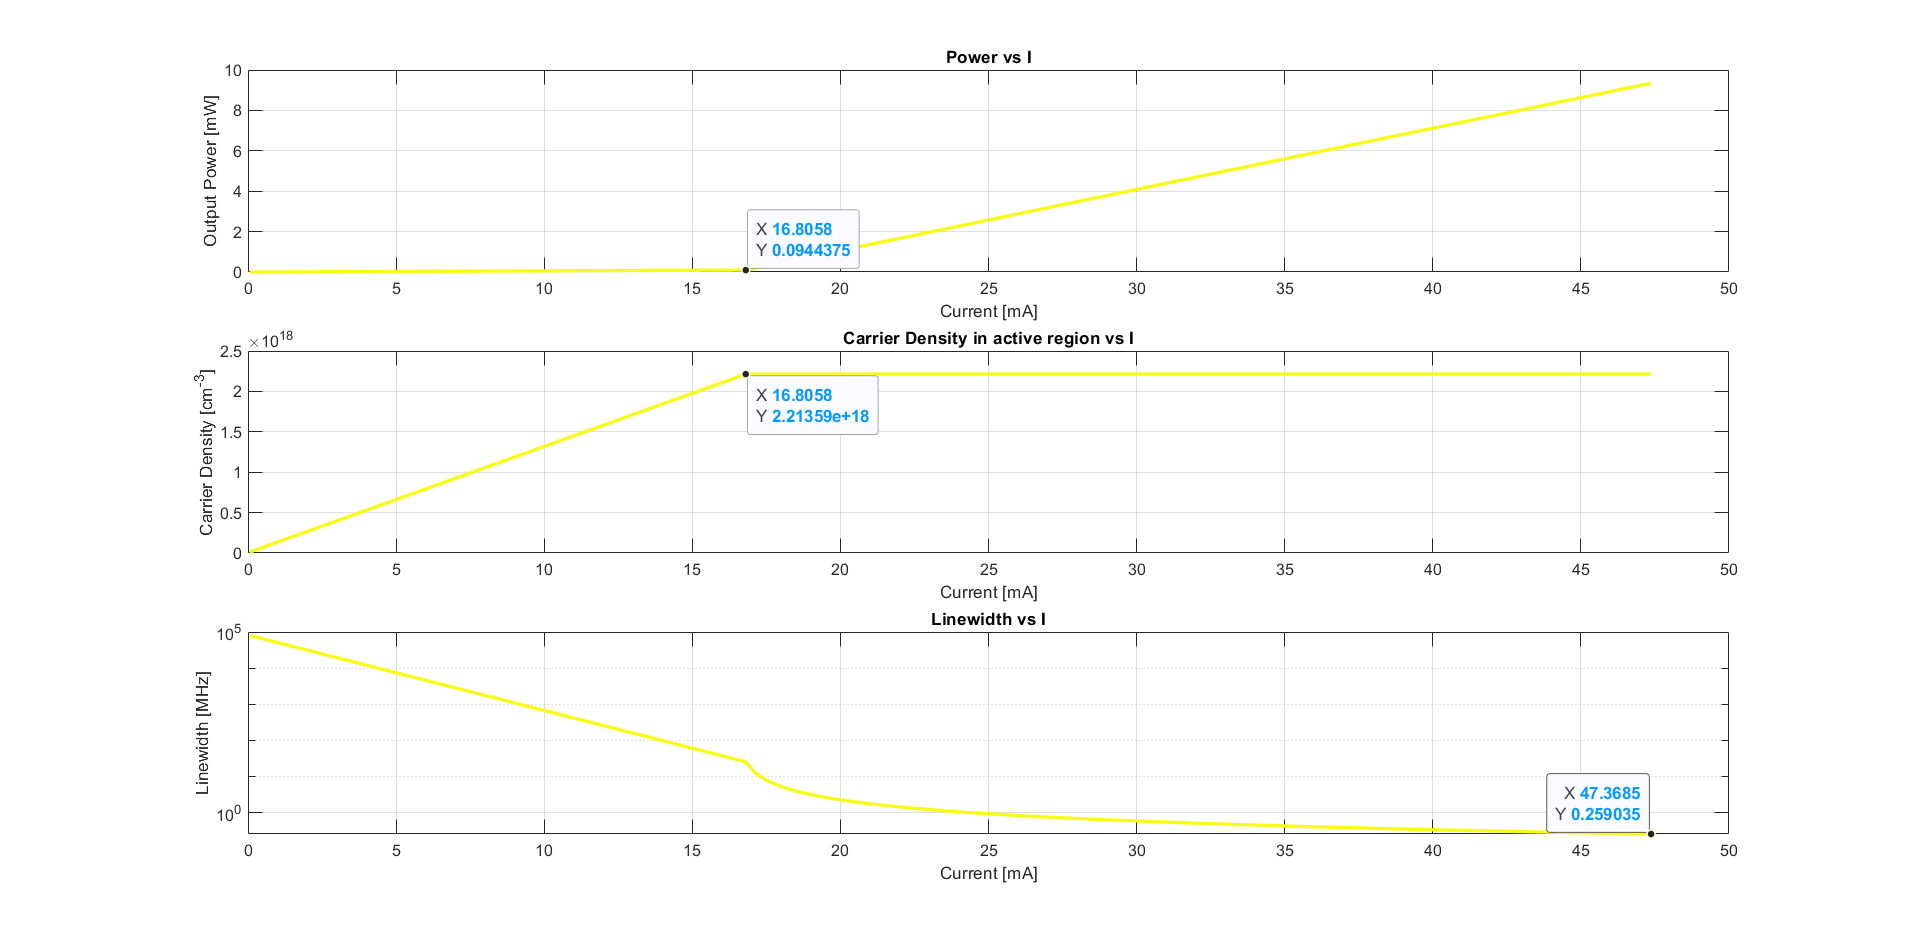
\includegraphics[width=15cm]{lab3/Images/prob1/P_N_Lw_vs_I_ah0.png}
  \caption{Andamento di $P_{\text{out}}$, $N$ e $\Delta\nu$ per $\alpha_H = 0$}
  \label{fig:P_N_Lw_vs_I_ah0}
\end{figure}

\begin{figure}[!h]
 \centering
 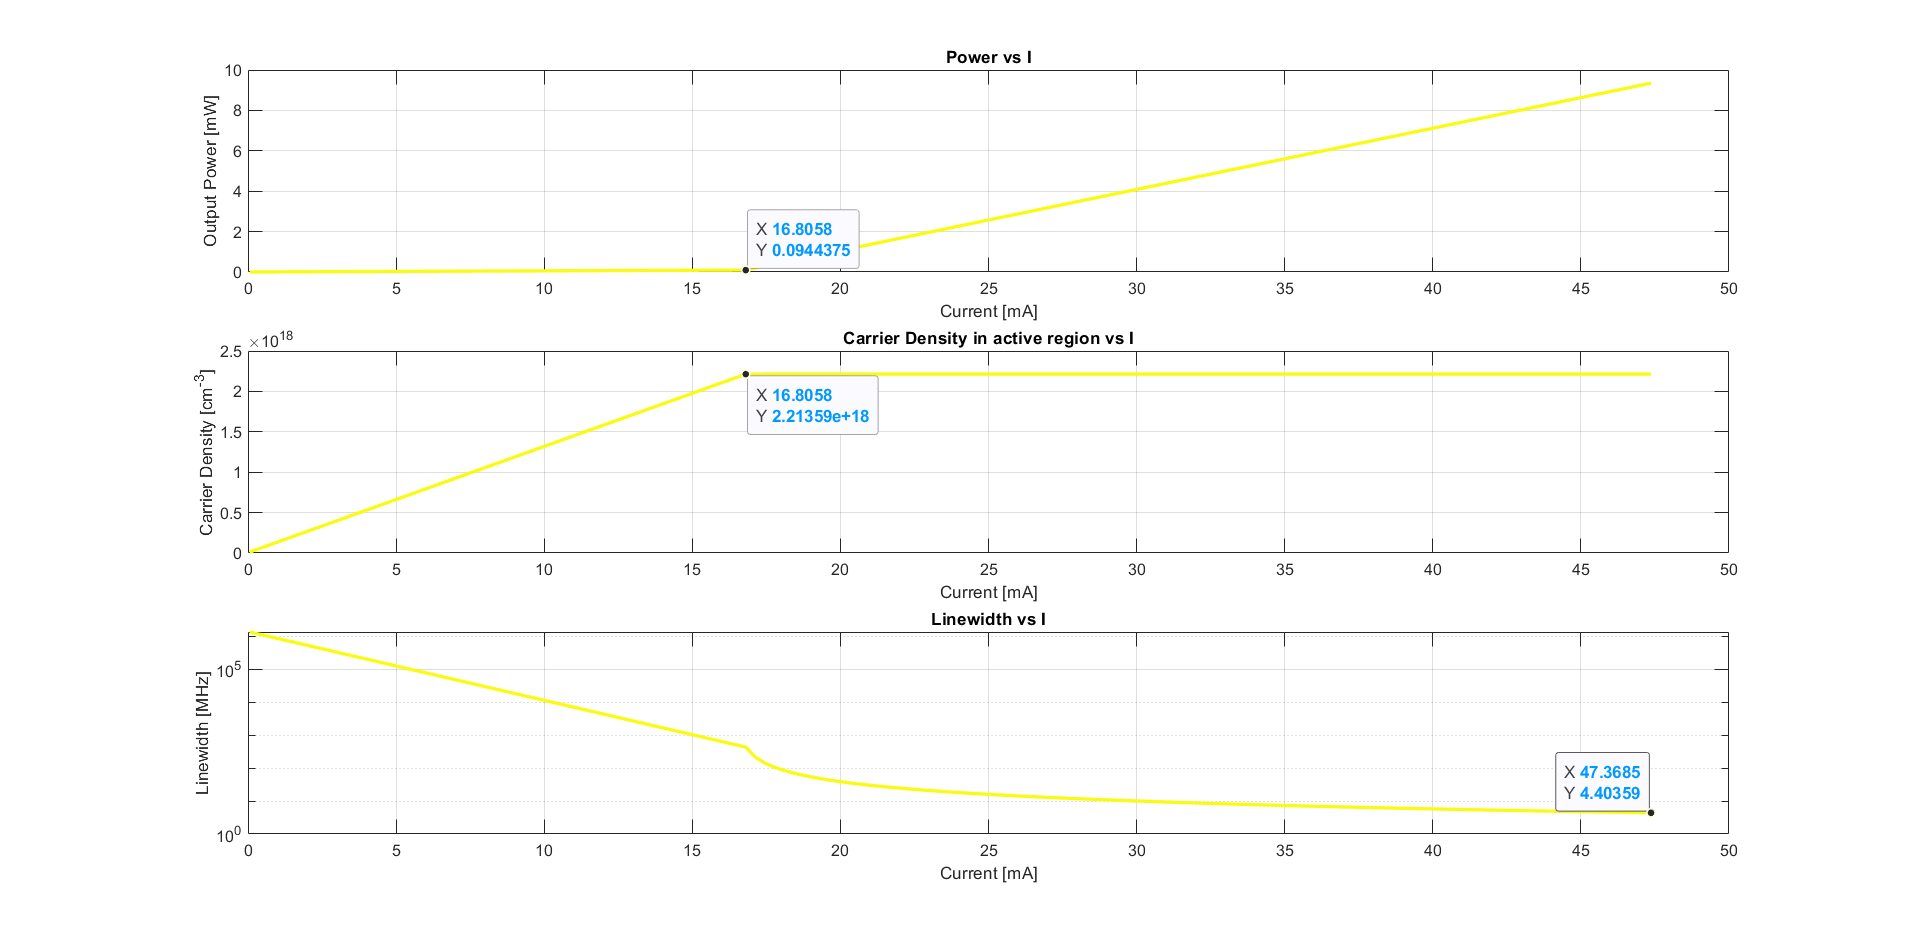
\includegraphics[width=15cm]{lab3/Images/prob1/P_N_Lw_vs_I_ah4.png}
  \caption{Andamento di $P_{\text{out}}$, $N$ e $\Delta\nu$ per $\alpha_H = 4$}
  \label{fig:P_N_Lw_vs_I_ah4}
\end{figure}

\noindent I calcoli teorici, effettuati con le relazioni illustrate in precedenza, portano ai seguenti risultati:
\[
    \Delta\nu_{FW,teor} (@ \alpha_H = 0) = \Delta\nu  \cdot (1 + 0^2) \approx 263.2 \text{ kHz}
\]
\[
    \Delta\nu_{FW,teor} (@ \alpha_H = 4) = \Delta\nu  \cdot (1 + 4^2) \approx 4.474 \text{ MHz}
\]

\noindent I valori stimati dal simulatore per i due casi di studio sono:
\[
    \Delta\nu_{FW,sim} (@ \alpha_H = 0) \approx 0.2590 \text{ MHz} \approx 259 \text{ kHz}
\]
\[
    \Delta\nu_{FW,sim} (@ \alpha_H = 4) \approx 4.404 \text{ MHz}
\] 

\newpage
\noindent Tutti i valori calcolati e stimati sono riassunti in Tabella \ref{tab:linewidth_comparison}.

\begin{table}[!h]
\centering
\begin{tabular}{|c|c|c|c|}
\hline
\textbf{$\boldsymbol{\Delta\nu_{FW}}$} & \textbf{Valore Simulazione} & \textbf{Valore Teorico} & \textbf{Errore [\%]} \\ \hline\hline
@ $\alpha_H = 0$ & $259$ kHz & $263.2$ kHz & 1.60 \% \\ \hline
@ $\alpha_H = 1$ & $518.1$ kHz & $526.4$ kHz & 1.58 \% \\ \hline
@ $\alpha_H = 4$ & $4.404$ MHz & $4.474$ MHz & 1.56 \% \\ \hline
\end{tabular}
\caption{Confronto tra i valori della larghezza di riga ottica del laser $\Delta\nu_{FW}$ stimati dal simulatore e quelli calcolati teoricamente per diversi valori di $\alpha_H$}
\label{tab:linewidth_comparison}
\end{table} 

\noindent Dalla comparazione dei valori teorici e simulati, si osserva un ottimo accordo tra i due approcci, con discrepanze minime (circa $1.58\%$). In particolare,
si nota come l'azzeramento del LEF ($\alpha_H = 0$) comporti una riduzione della larghezza di riga spettrale di un fattore 2 rispetto al caso con $\alpha_H = 1$.

\noindent\\ Al contrario, l'aumento del LEF ($\alpha_H = 4$) comporta un incremento significativo della larghezza di riga, di circa un fattore $8.5$ rispetto al caso nominale
con $\alpha_H = 1$, determinando un significativo aumento della larghezza di riga e una conseguente riduzione della coerenza temporale. Tale incremento è dovuto proprio al
termine $1 + \alpha_H^2$, che cresce in modo quadratico con l'aumentare del LEF, amplificando l'effetto del rumore di fase indotto dalle fluttuazioni di intensità.

\newpage
\section{Risposte IM e FM del diodo laser}
Il secondo assignment del laboratorio prevede l'analisi dinamica a piccolo segnale del diodo laser, valutata per diverse correnti di bias, al fine di evidenziare le
caratteristiche e le differenze fondamentali tra la risposta di modulazione di intensità (IM) e quella di frequenza (FM).

\subsection{Risposta temporale della dinamica a piccolo segnale}
\noindent Per lo studio della dinamica a piccolo segnale, il dispositivo è stato caratterizzato in corrispondenza di quattro diversi punti di lavoro sopra soglia:\\
$I_{\text{bias,1}} = 2 \cdot I_{\text{th}}$, $I_{\text{bias,2}} = 1.05 \cdot I_{\text{th}}$, $I_{\text{bias,3}} = 6 \cdot I_{\text{th}}$ e $I_{\text{bias,4}} = 10 \cdot I_{\text{th}}$.

\noindent L'analisi di queste quattro condizioni operative consente di osservare come la risposta dinamica del laser si modifichi al variare del livello di iniezione
dei portatori, evidenziando l'evoluzione della frequenza di risonanza delle oscillazioni di rilassamento ($f_r$), dell'effetto di smorzamento (\textit{damping}) e della
banda di modulazione a $-3\text{ dB}$ sia per la risposta IM che per quella FM.
\noindent Gli andamenti della potenza ottica $P$, della densità di portatori $N$ e dell'allargamento di riga $\Delta\nu$ in funzione del tempo sono riportati nelle seguenti Figure.

\begin{figure}[!h]
 \centering
 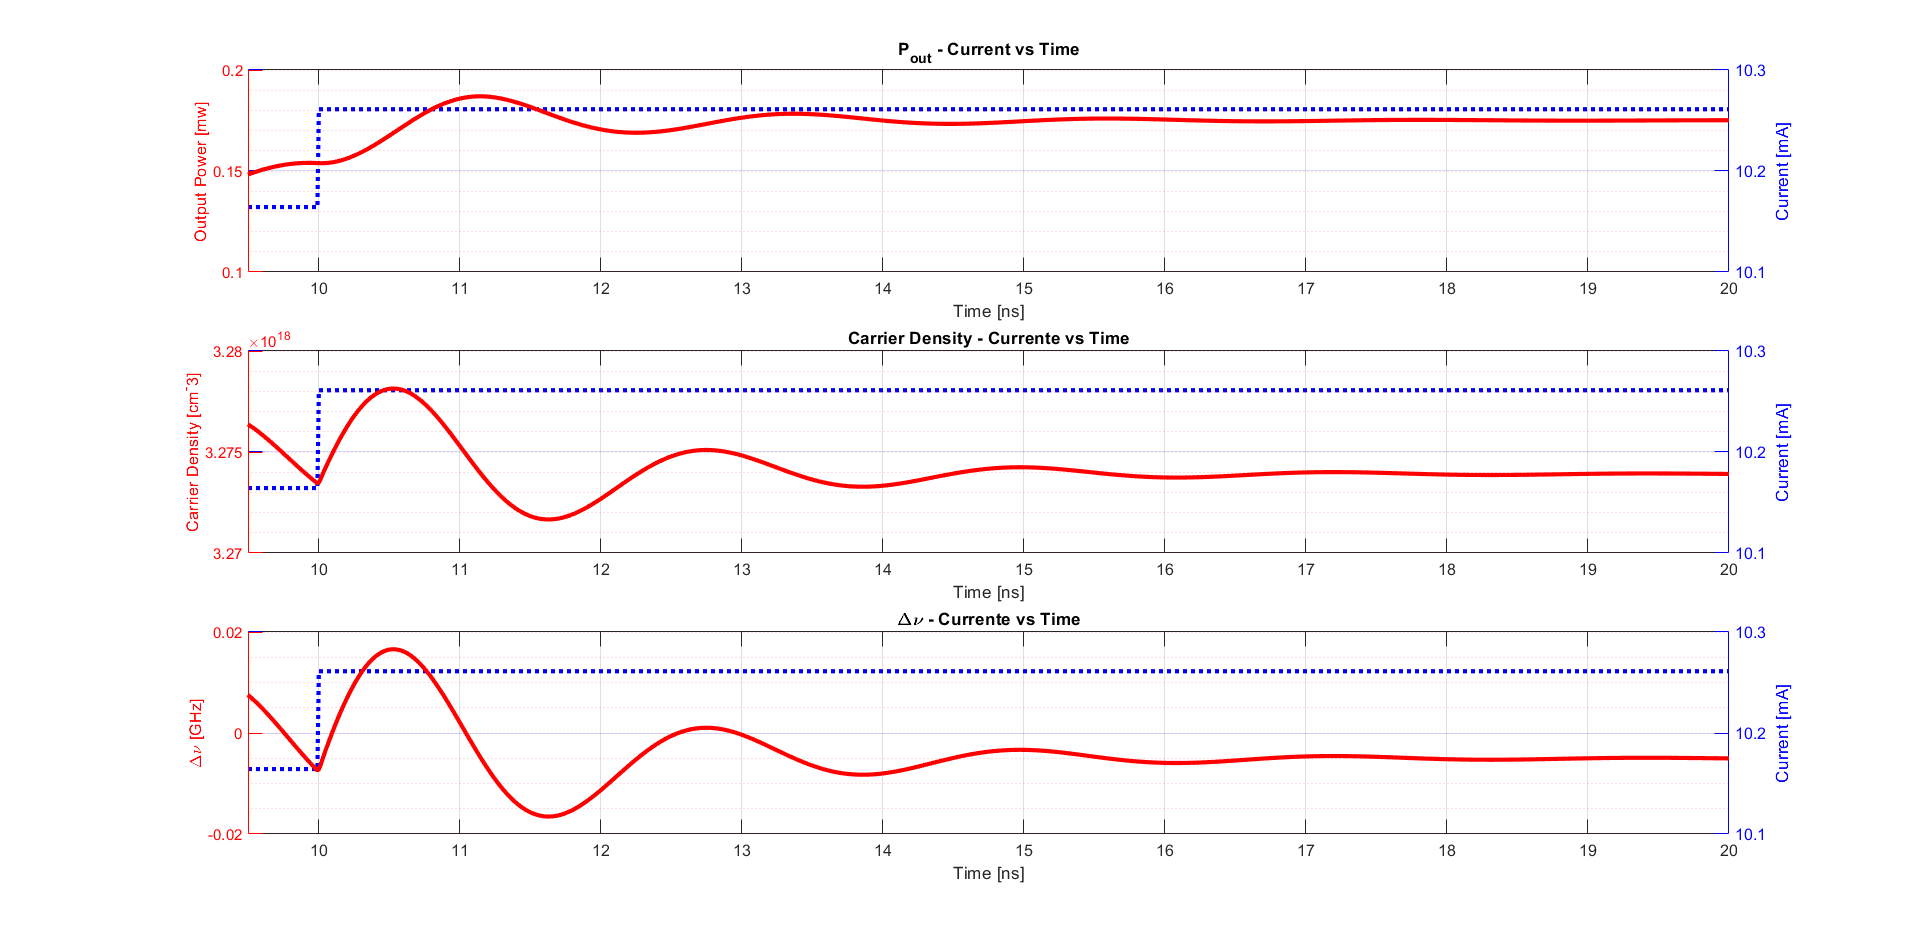
\includegraphics[width=15cm]{lab3/Images/prob2/P_N_vs_t_1_05.png}
  \caption{Analisi dinamica per $I_{\text{bias}} = 1.05 \cdot I_{\text{th}}$}
  \label{fig:P_N_vs_t_1_05}
\end{figure}

\begin{figure}[!h]
 \centering
 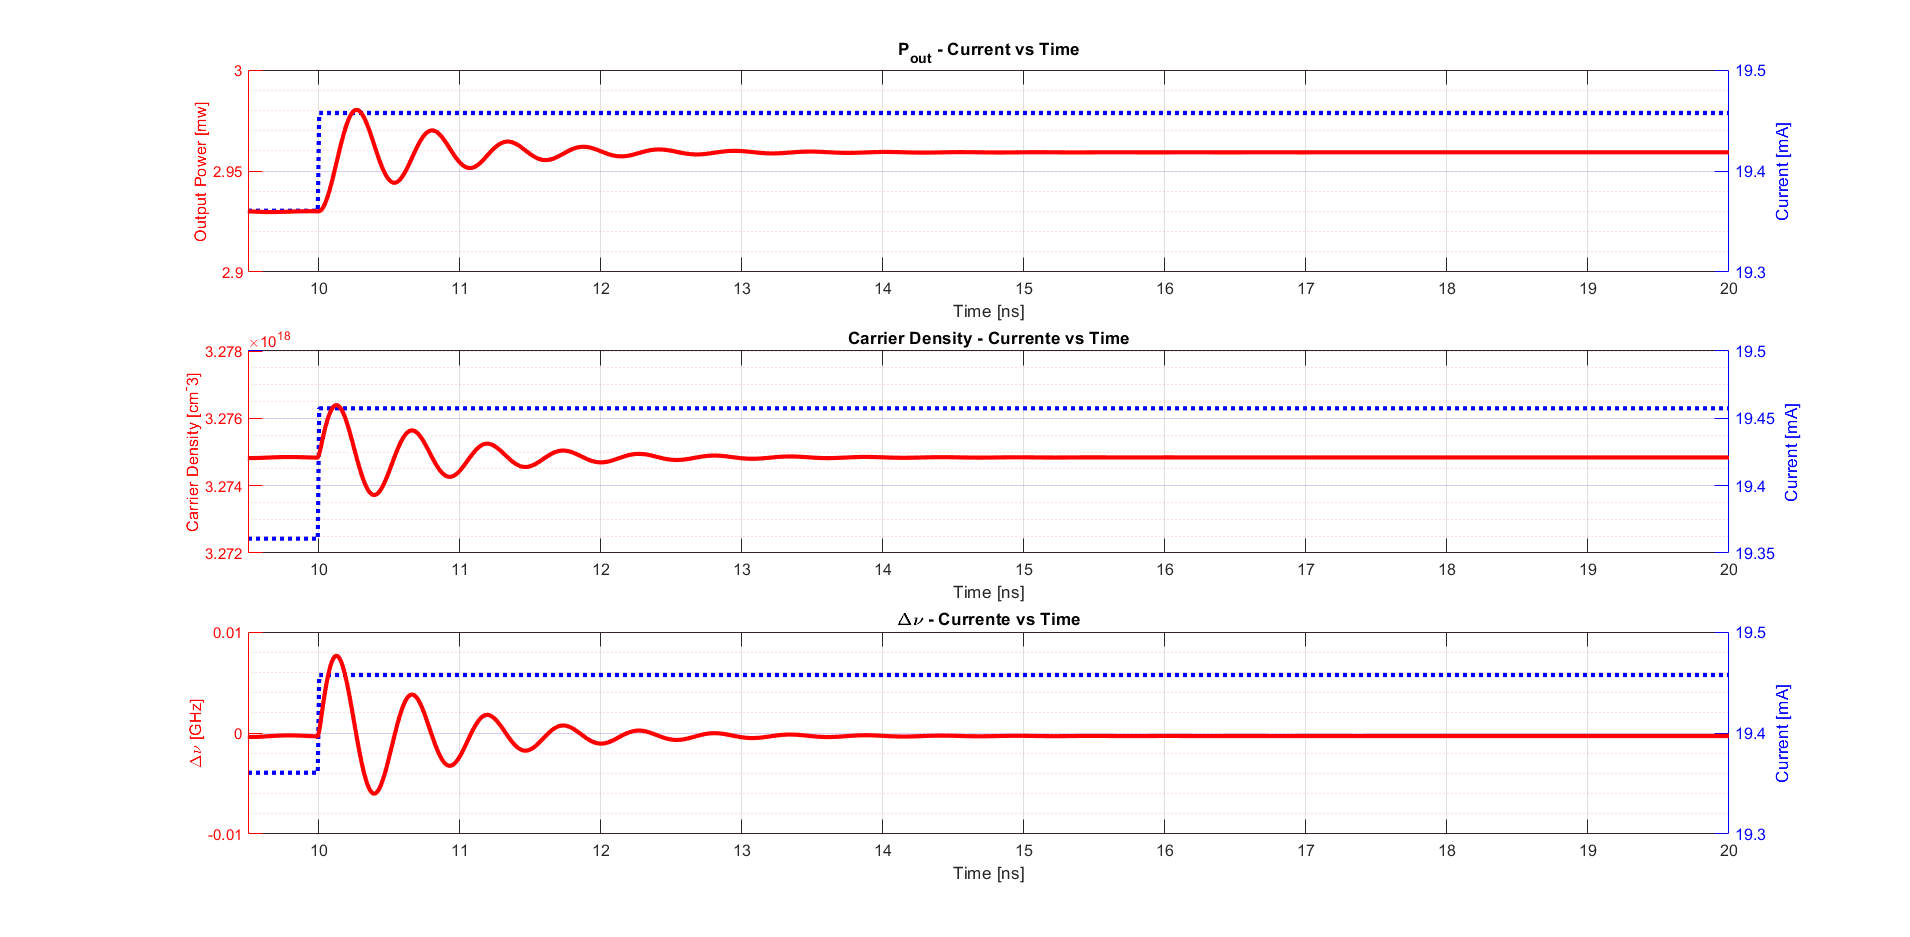
\includegraphics[width=15cm]{lab3/Images/prob2/P_N_vs_t_2.png}
  \caption{Analisi dinamica per $I_{\text{bias}} = 2 \cdot I_{\text{th}}$}
  \label{fig:P_N_vs_t_2}
\end{figure}

Nelle Figure \ref{fig:P_N_vs_t_1_05} e \ref{fig:P_N_vs_t_2}, relative a correnti di polarizzazione prossime al valore di soglia, si osserva un transitorio prolungato
caratterizzato da oscillazioni di rilassamento marcate prima del raggiungimento dello stato stazionario.

\begin{figure}[!h]
 \centering
 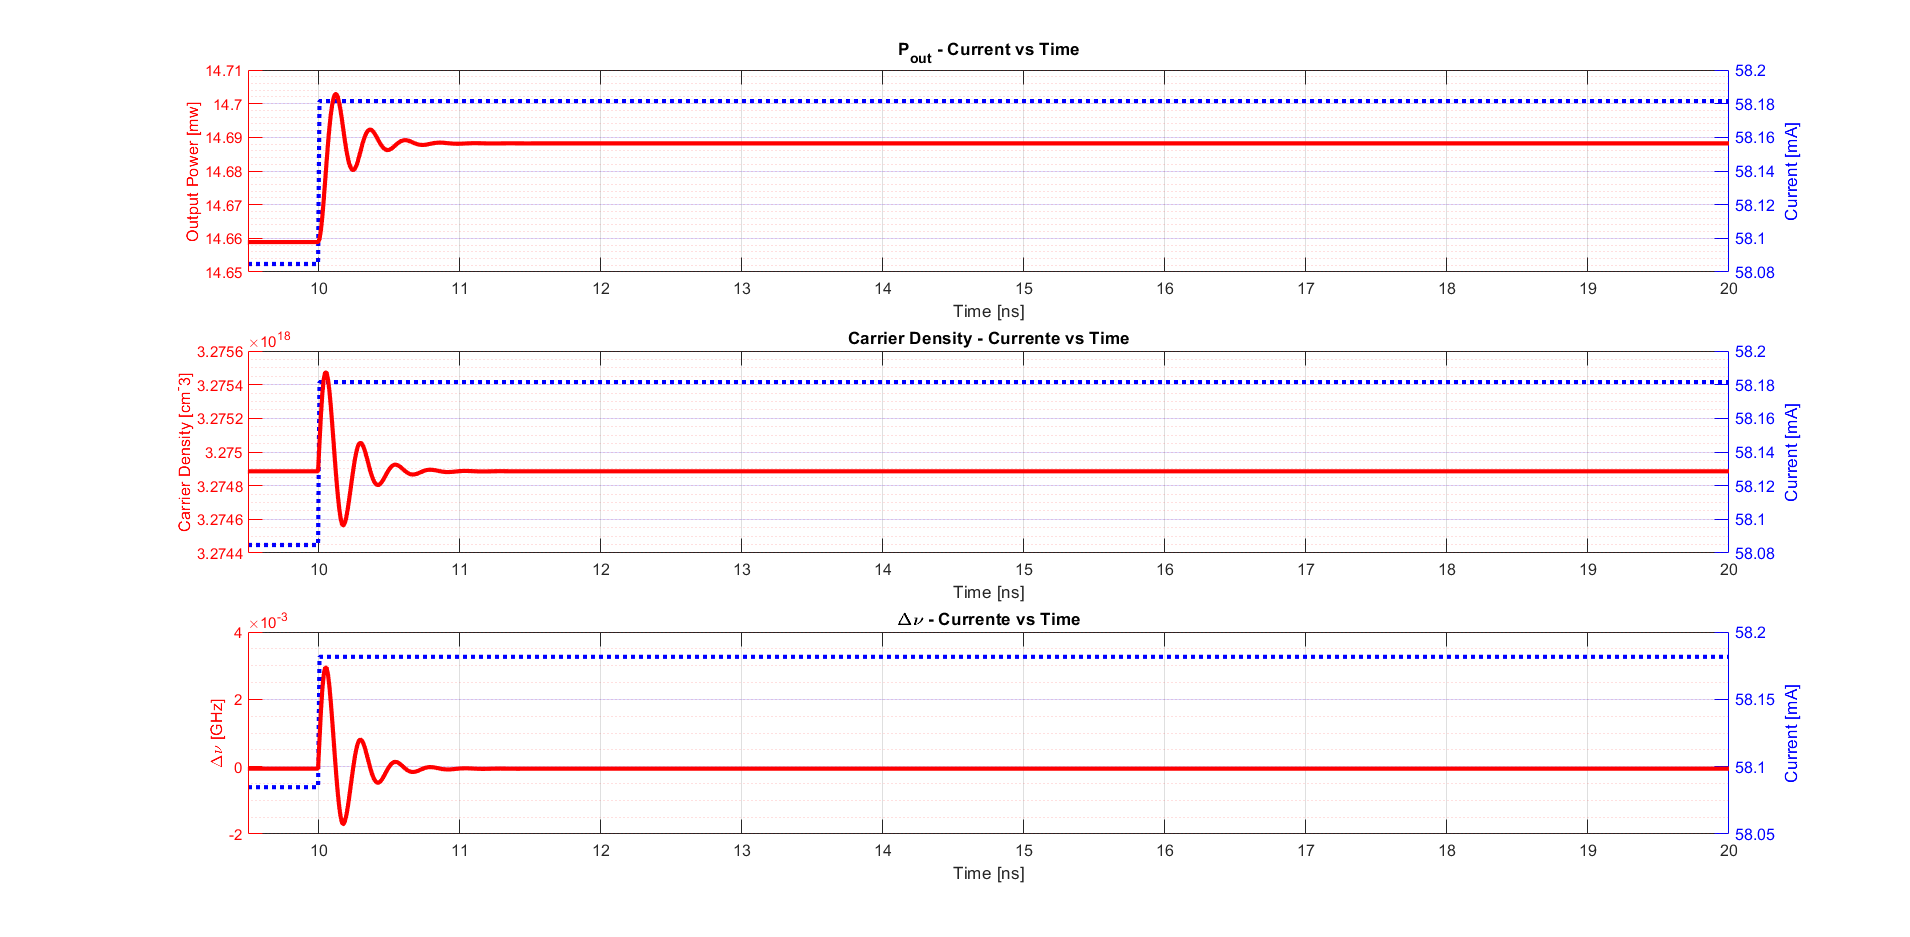
\includegraphics[width=15cm]{lab3/Images/prob2/P_N_vs_t_6.png}
  \caption{Analisi dinamica per $I_{\text{bias}} = 6 \cdot I_{\text{th}}$}
  \label{fig:P_N_vs_t_6}
\end{figure}

\begin{figure}[!h]
 \centering
 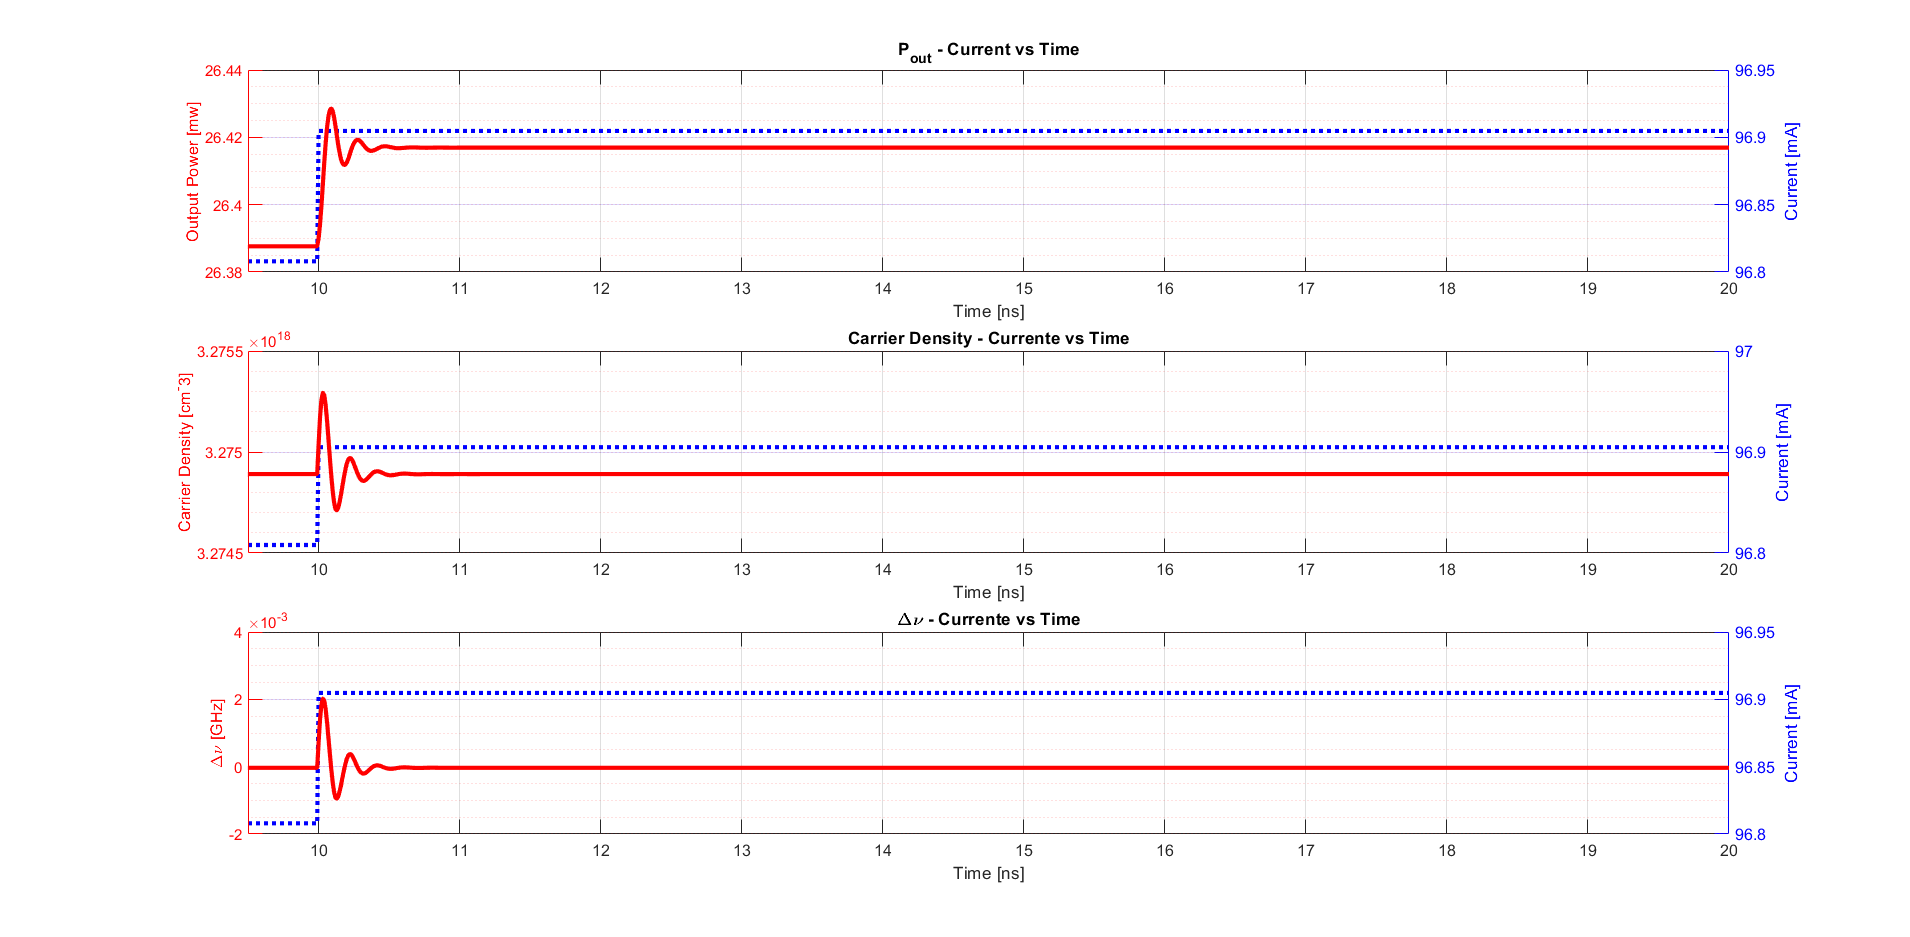
\includegraphics[width=15cm]{lab3/Images/prob2/P_N_vs_t_10.png}
  \caption{Analisi dinamica per $I_{\text{bias}} = 10 \cdot I_{\text{th}}$}
  \label{fig:P_N_vs_t_10}
\end{figure}

\noindent Con correnti di bias molto maggiori della corrente di soglia $I_{\text{th}}$ (Figure \ref{fig:P_N_vs_t_6} e \ref{fig:P_N_vs_t_10}), la frequenza delle oscillazioni aumenta
e lo smorzamento diventa più efficace, riducendo nettamente la durata del transitorio per tutte le grandezze considerate. In generale, l'aumento della corrente di bias
velocizza la risposta del dispositivo e ne migliora la dinamica temporale.

\noindent\\ La riduzione della durata del transitorio e il contestuale aumento della frequenza delle oscillazioni all'aumentare della corrente di polarizzazione trovano
diretta spiegazione nell'analisi a piccolo segnale delle \textit{rate equations}. \\
Dai termini della matrice di risposta, la frequenza angolare delle oscillazioni di rilassamento $\omega_R$ (e quindi $f_r$) risulta proporzionale alla radice
quadrata della densità di fotoni stazionaria $N_p$:
\begin{equation}
f_r = \frac{\omega_R}{2\pi} \approx  \frac{1}{2\pi} \sqrt{\frac{v_g a N_p}{\tau_p}} \propto \sqrt{I_{\text{bias}} - I_{\text{th}}}
\end{equation}
dove $a$ rappresenta il guadagno differenziale e $\tau_p$ il tempo di vita dei fotoni nella cavità.

\noindent\\ Contemporaneamente, l'aumento della corrente sopra soglia incrementa il fattore di smorzamento del sistema:
\begin{equation}
\gamma \approx  v_g a N_p \left[1+ \frac{\Gamma a_p}{a} \right] + \frac{1}{\tau_{\Delta n}} \propto I_{\text{bias}} - I_{\text{th}}
\end{equation} 
L'effetto combinato
dell'aumento di $f_r$ e di $\gamma$ velocizza la dinamica del sistema e smorza più rapidamente le oscillazioni di rilassamento, riducendo la durata del transitorio di
accensione e stabilizzando il laser sul valore stazionario in tempi più brevi.

\noindent\\ A partire da questa caratterizzazione nel dominio del tempo, si è proceduto con la simulazione della risposta in frequenza a piccolo segnale per la modulazione di intensità
(IM) e di frequenza (FM) nei quattro punti di lavoro.

\noindent\\
\subsection{Risposta in frequenza - Plot IM e FM}
Nelle pagine seguenti vengono riportati i grafici della risposta in frequenza a piccolo segnale per la modulazione di intensità (IM) e di frequenza (FM) del diodo laser,
ottenuti per le quattro correnti di bias considerate. In tutti i casi considerati è stato impostato un valore di \textit{Gain Compression Factor} pari a $\epsilon_1 = 0$.

\begin{figure}[!h]
    \centering
    \begin{subfigure}[b]{0.49\textwidth}
        \centering
        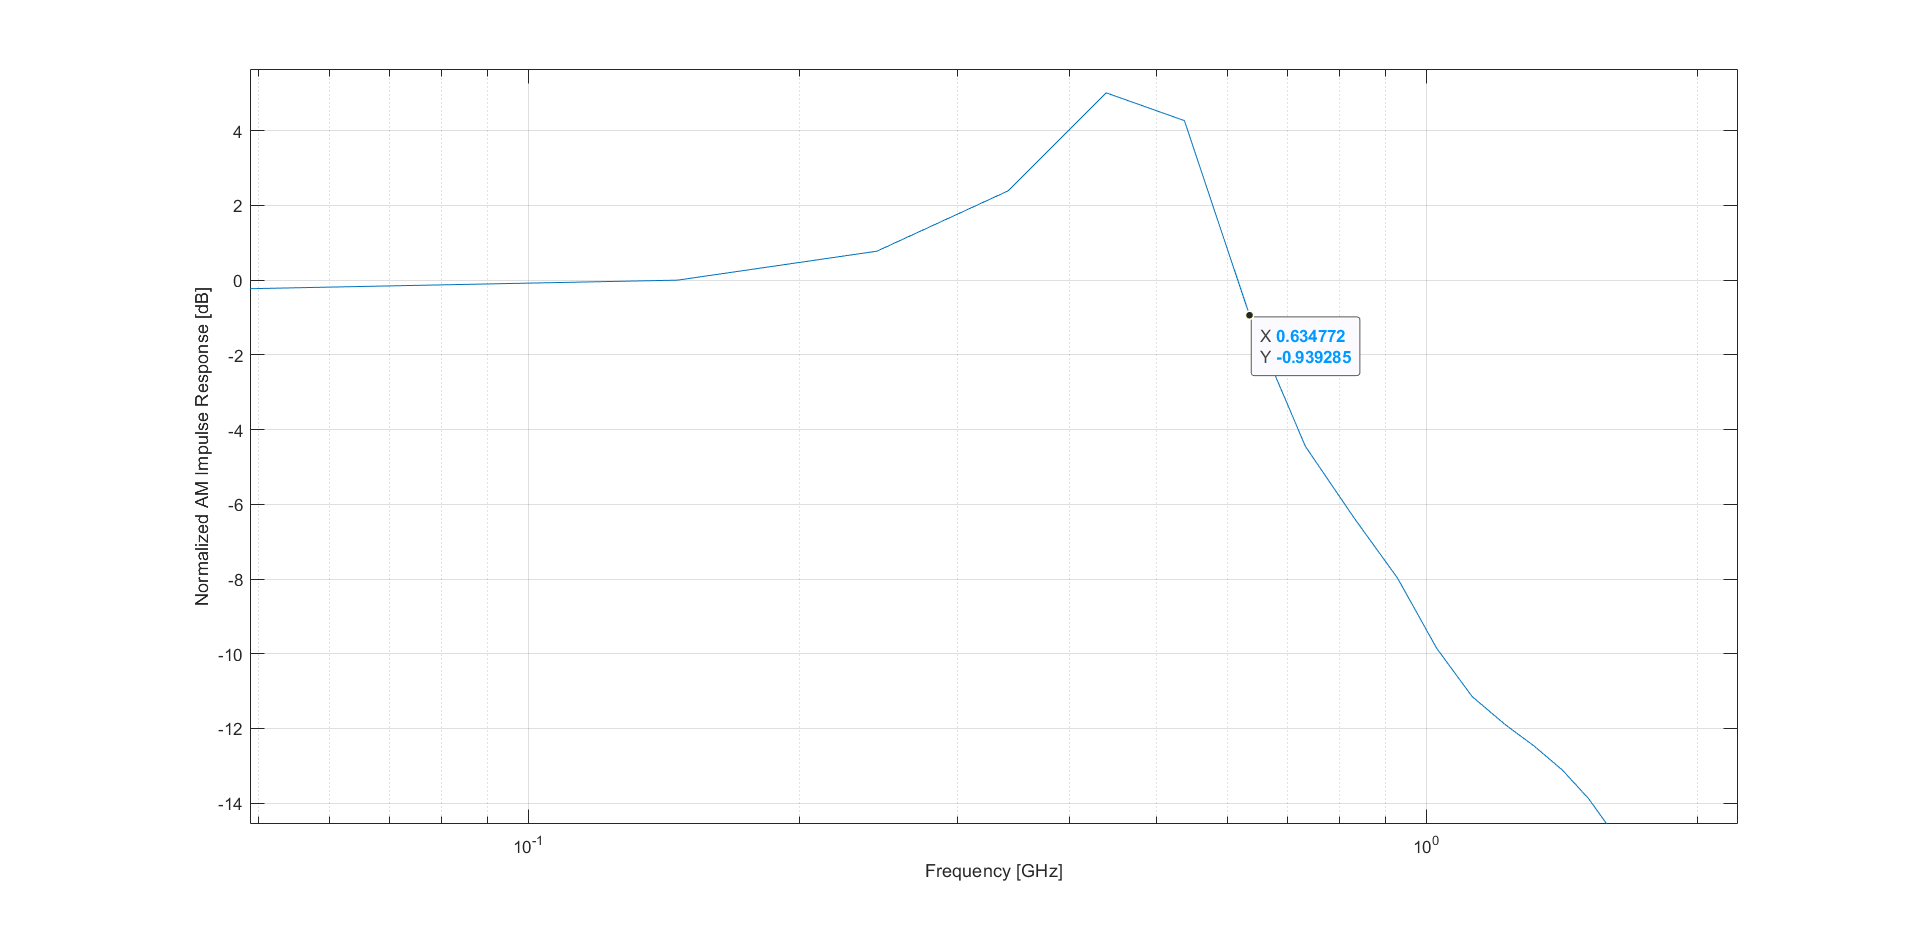
\includegraphics[width=\textwidth]{lab3/Images/prob2/IM_1_05.png}
        \caption{Risposta IM del laser con $I_b = 1.05 I_{\text{th}}$}
        \label{fig:IM_1_05}
    \end{subfigure}
    \hfill
    \begin{subfigure}[b]{0.49\textwidth}
        \centering
        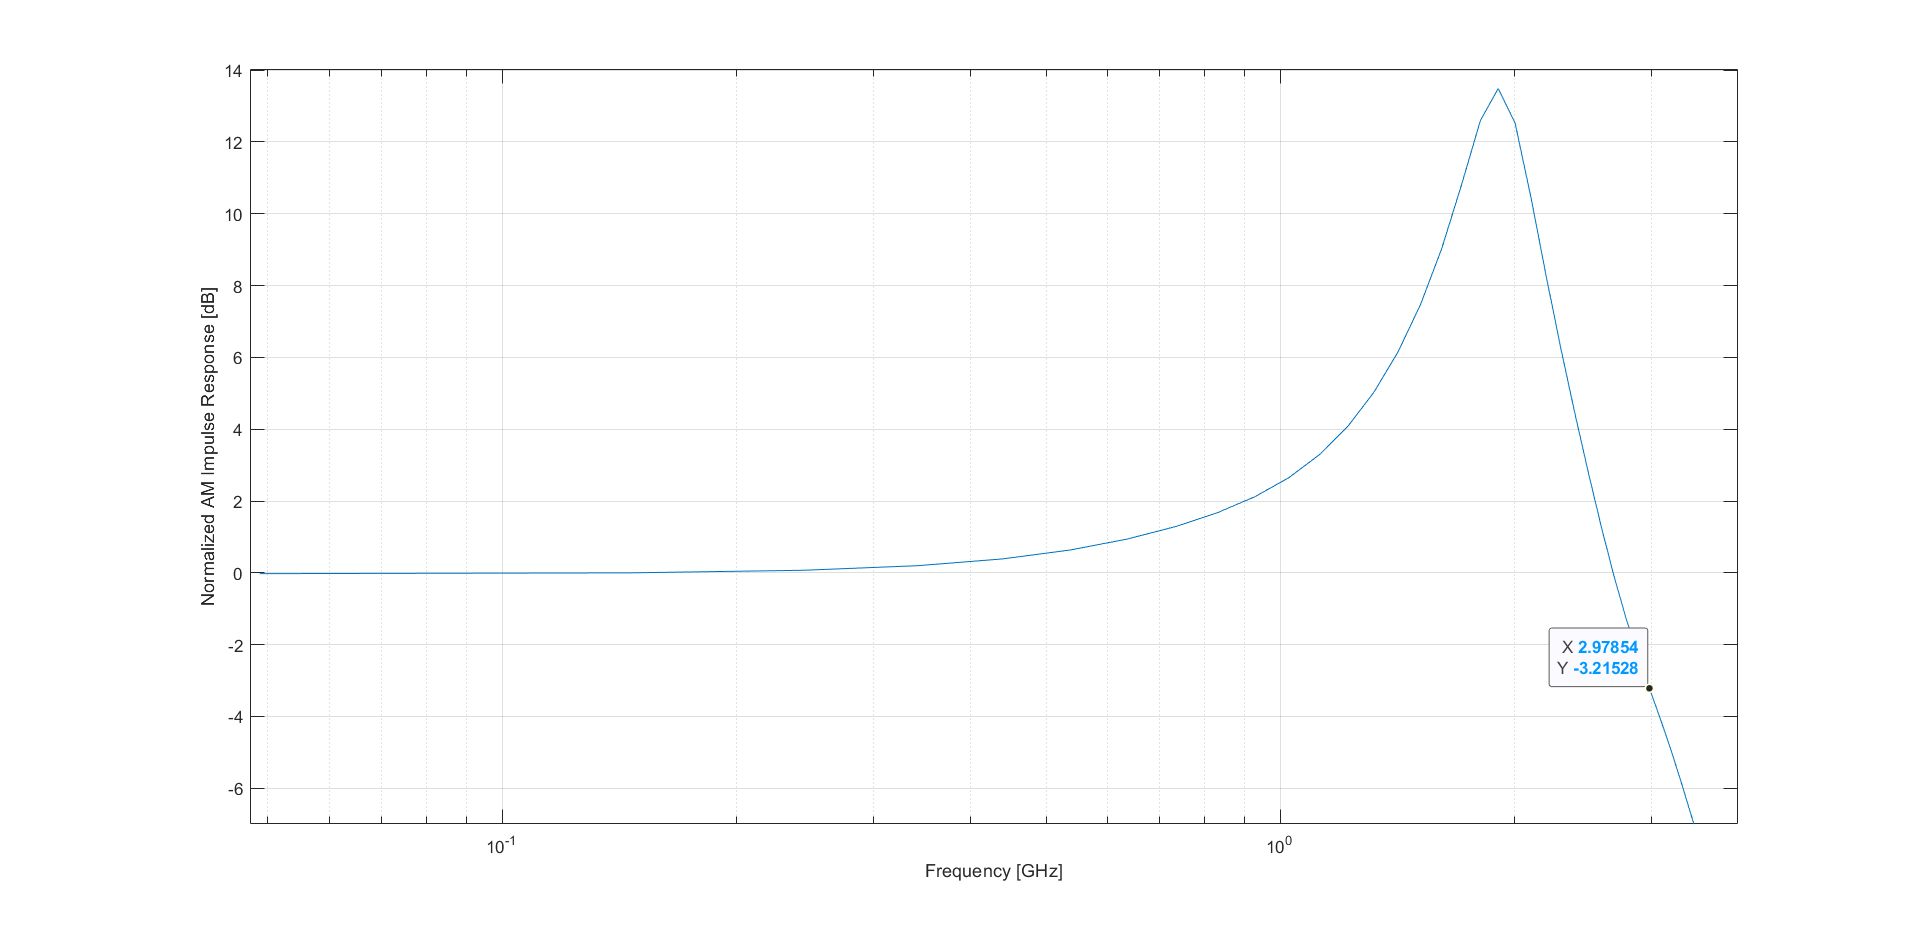
\includegraphics[width=\textwidth]{lab3/Images/prob2/IM_2.png}
        \caption{Risposta IM del laser con $I_b = 2 I_{\text{th}}$}
        \label{fig:IM_2}
    \end{subfigure}
    \caption{Risposta IM del laser con correnti di polarizzazione $I_b = 1.05 I_{\text{th}}$ e $I_b = 2 I_{\text{th}}$}
    \label{fig:IM_b1_b2}
\end{figure}


\begin{figure}[!h]
    \centering
    \begin{subfigure}[b]{0.49\textwidth}
        \centering
        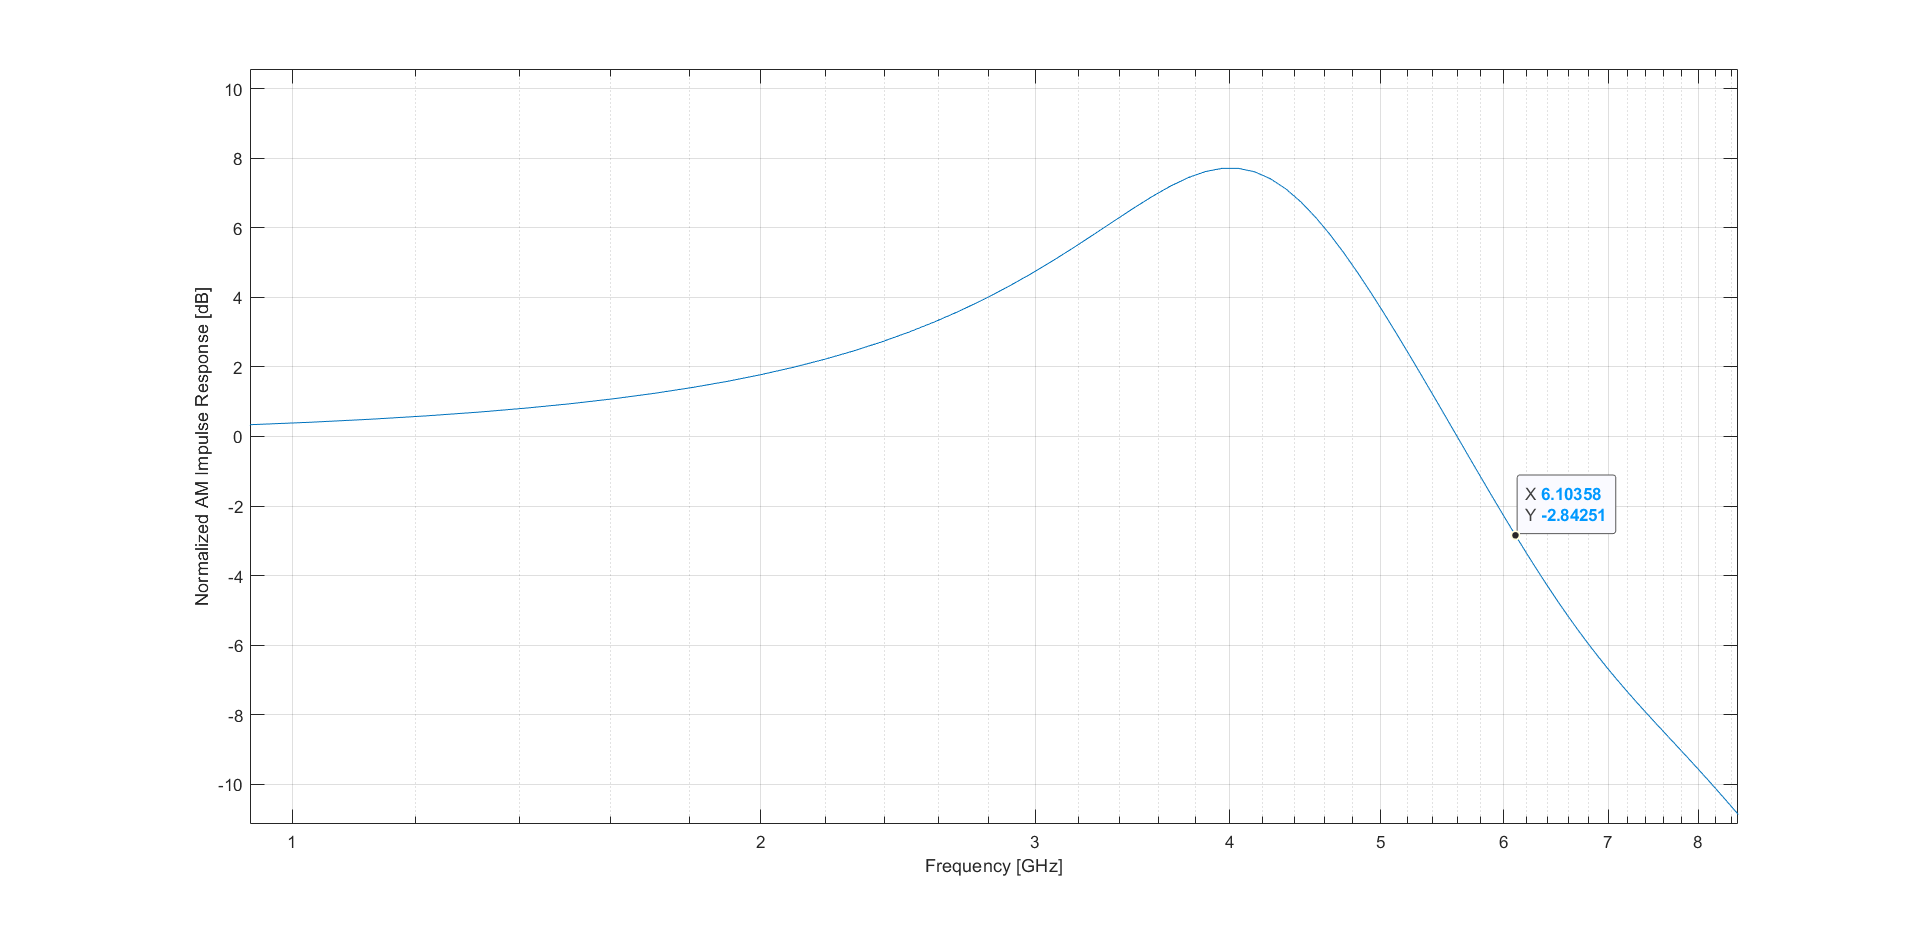
\includegraphics[width=\textwidth]{lab3/Images/prob2/IM_6.png}
        \caption{Risposta IM del laser con $I_b = 6 I_{\text{th}}$}
        \label{fig:IM_6}
    \end{subfigure}
    \hfill
    \begin{subfigure}[b]{0.49\textwidth}
        \centering
        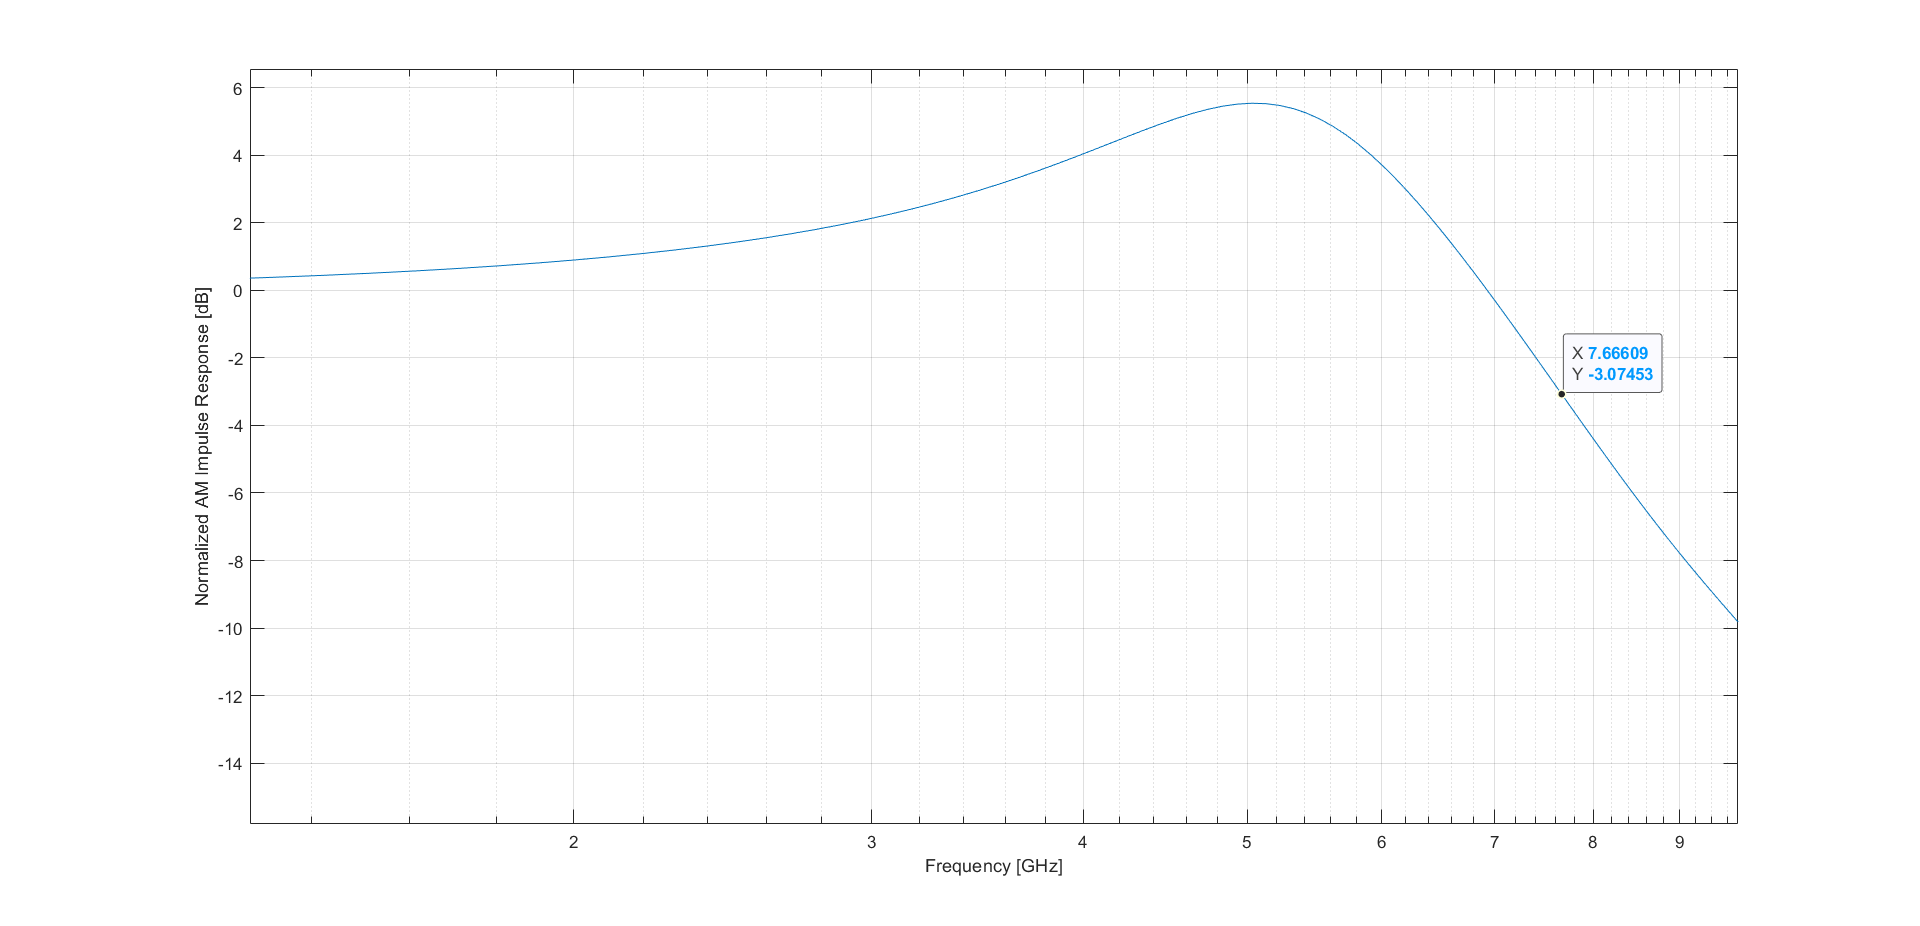
\includegraphics[width=\textwidth]{lab3/Images/prob2/IM_10.png}
        \caption{Risposta IM del laser con $I_b = 10 I_{\text{th}}$}
        \label{fig:IM_10}
    \end{subfigure}
    \caption{Risposta IM del laser con correnti di polarizzazione $I_b = 6 I_{\text{th}}$ e $I_b = 10 I_{\text{th}}$}
    \label{fig:IM_b3_b4}
\end{figure}

\noindent Come ci si aspetterebbe dalla teoria, la risposta è del tipo passa-basso del secondo ordine con una coppia di poli complessi coniugati (che danno origine al picco
di risonanza); misurando la banda a $-3\text{ dB}$ dai grafici sopra riportati, otteniamo i risultati riportati in Tabella \ref{tab:bandaAM_3dB}, che evidenziano come la
banda di modulazione aumenti all'aumentare della corrente di bias.

\begin{table}[!h]
    \centering
    \begin{tabular}{c c}
        \hline
        \textbf{Corrente di bias ($I_{\text{bias}}$)} & \textbf{Banda AM a $-3\text{ dB}$ ($f_{-3\text{dB}}$)} \\
        \hline
        $1.05 \, I_{\text{th}}$ & $680  \text{ MHz}$ \\
        $2.0 \, I_{\text{th}}$  & $2.90 \text{ GHz}$ \\
        $6.0 \, I_{\text{th}}$  & $6.20 \text{ GHz}$ \\
        $10.0 \, I_{\text{th}}$ & $7.65 \text{ GHz}$ \\
        \hline
    \end{tabular}
    \caption{Banda di modulazione AM a $-3\text{ dB}$ al variare della corrente di polarizzazione}
    \label{tab:bandaAM_3dB}
\end{table}

\newpage

\begin{figure}[!h]
    \centering
    \begin{subfigure}[b]{0.49\textwidth}
        \centering
        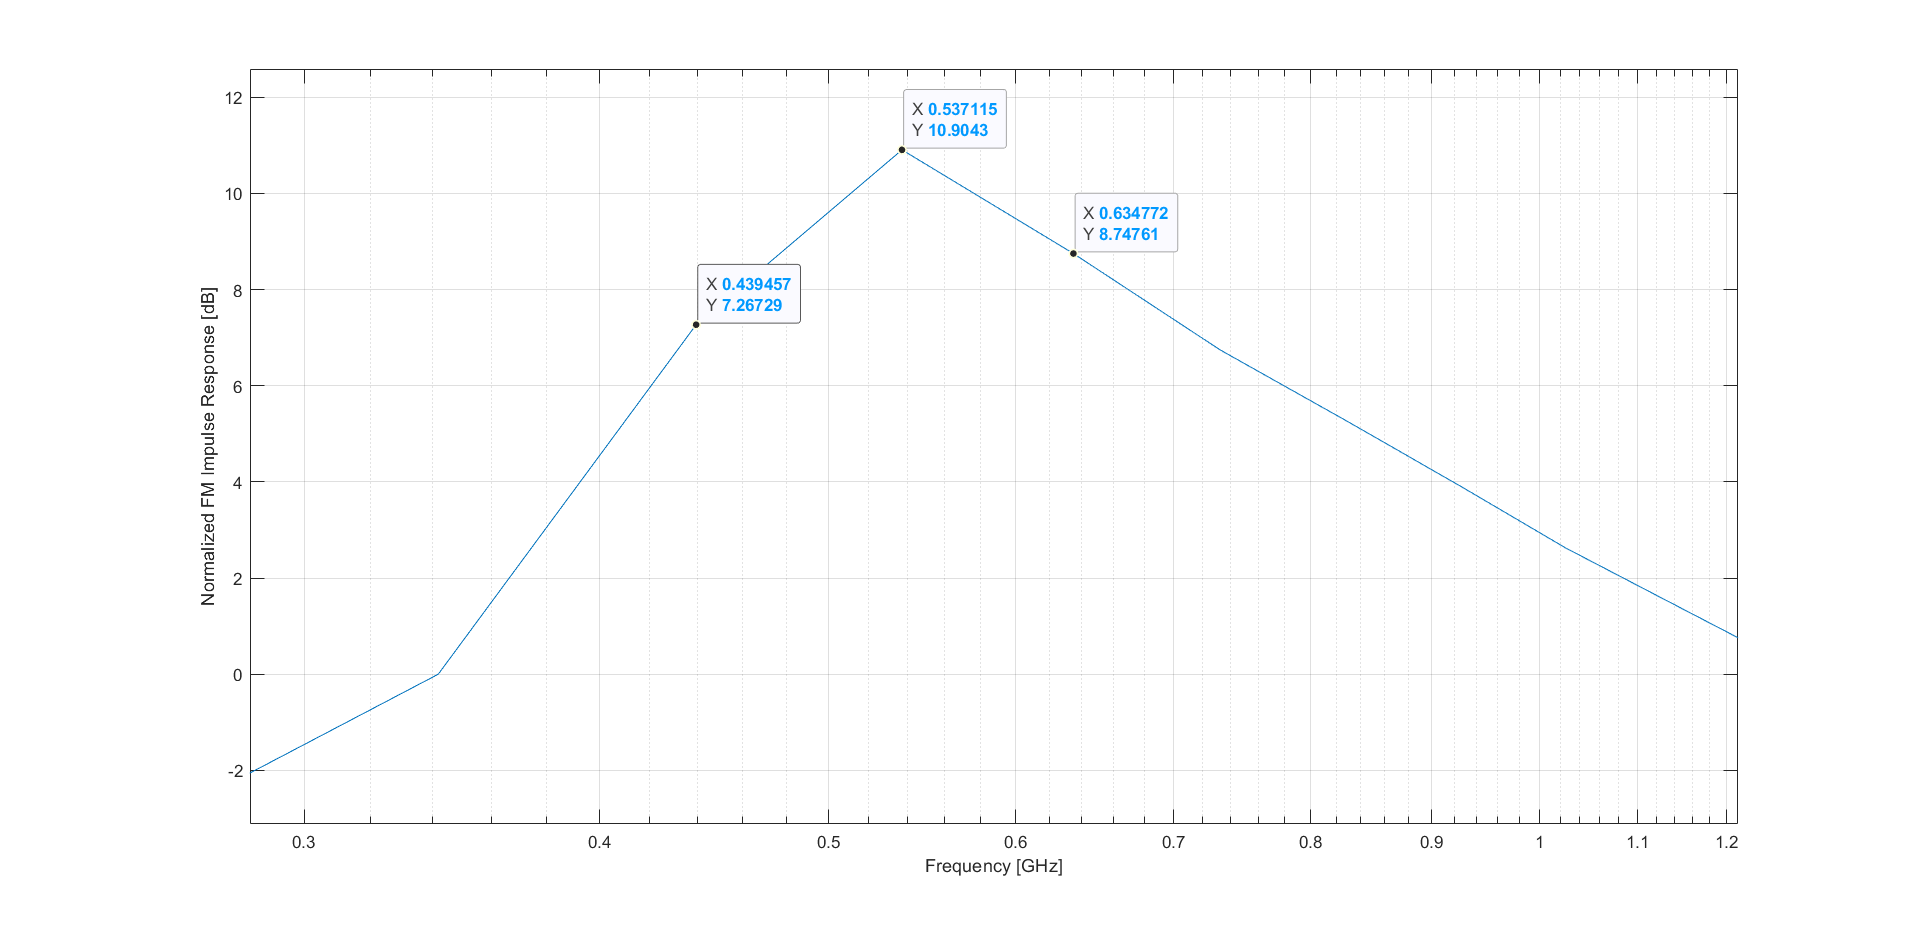
\includegraphics[width=\textwidth]{lab3/Images/prob2/FM_1_05.png}
        \caption{Risposta FM del laser con $I_b = 1.05 I_{\text{th}}$}
        \label{fig:FM_1_05}
    \end{subfigure}
    \hfill
    \begin{subfigure}[b]{0.49\textwidth}
        \centering
        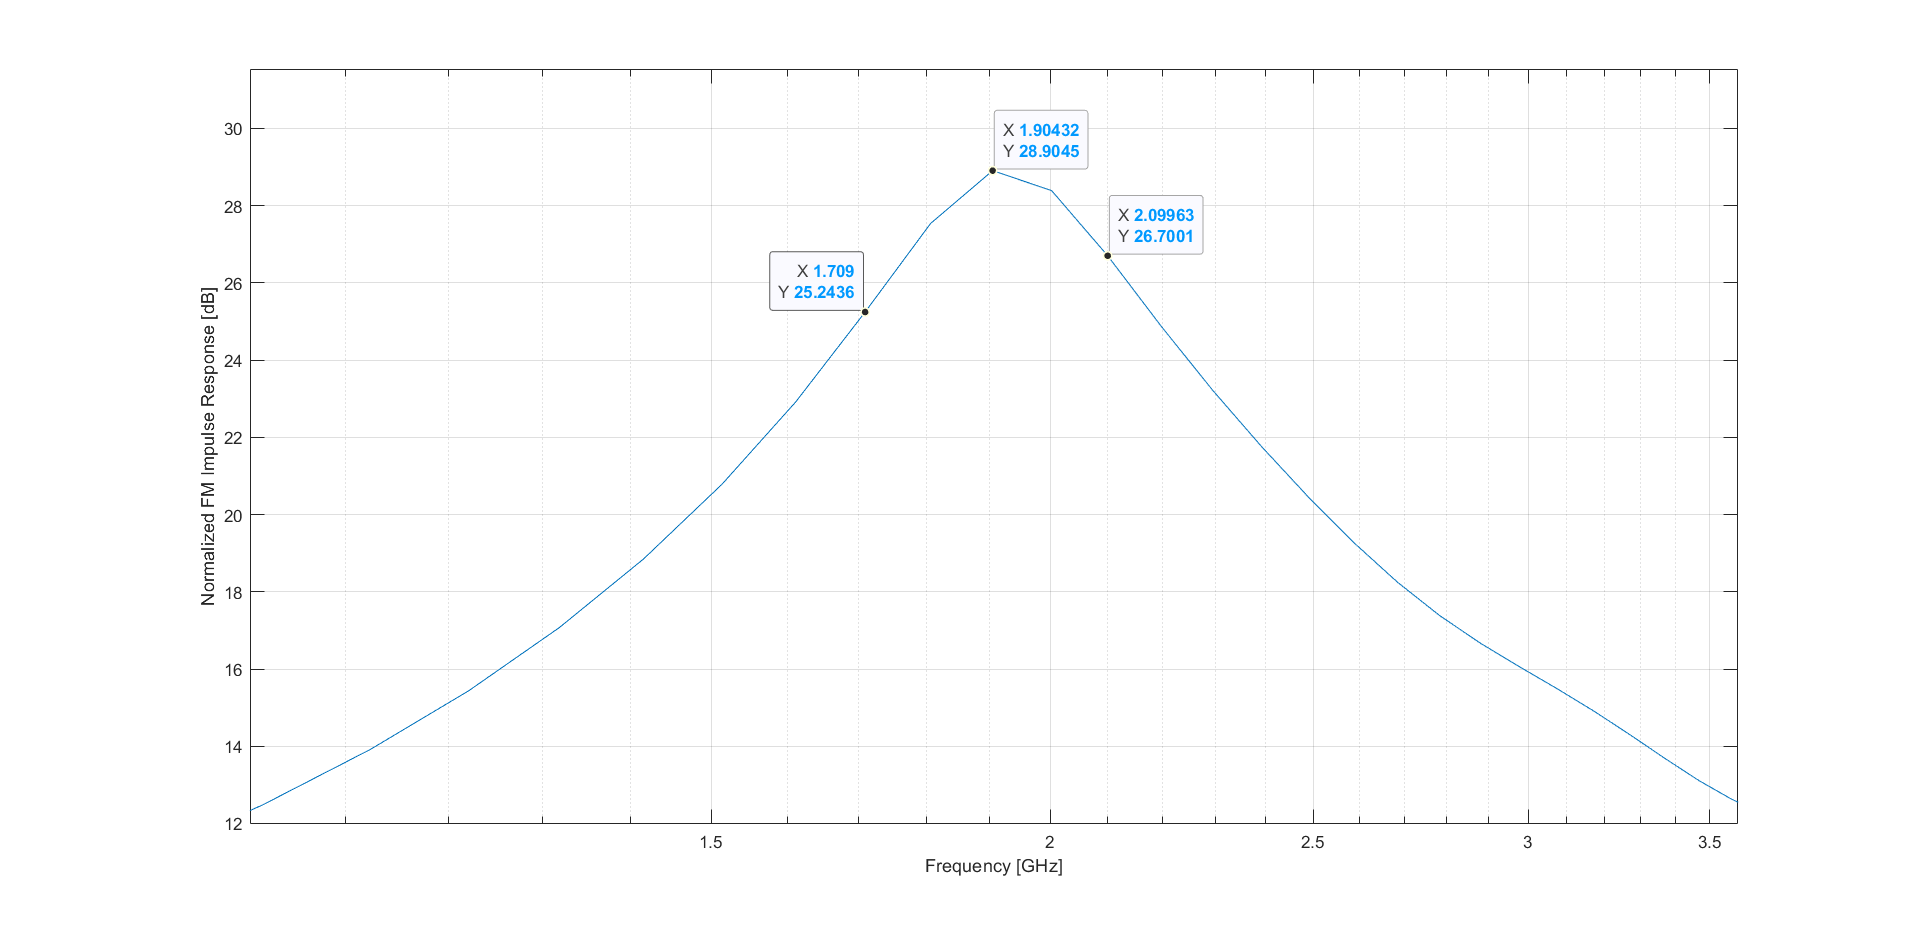
\includegraphics[width=\textwidth]{lab3/Images/prob2/FM_2.png}
        \caption{Risposta FM del laser con $I_b = 2 I_{\text{th}}$}
        \label{fig:FM_2}
    \end{subfigure}
    \caption{Risposta FM del laser con correnti di polarizzazione $I_b = 1.05 I_{\text{th}}$ e $I_b = 2 I_{\text{th}}$}
    \label{fig:FM_b1_b2}
\end{figure}


\begin{figure}[!h]
    \centering
    \begin{subfigure}[b]{0.49\textwidth}
        \centering
        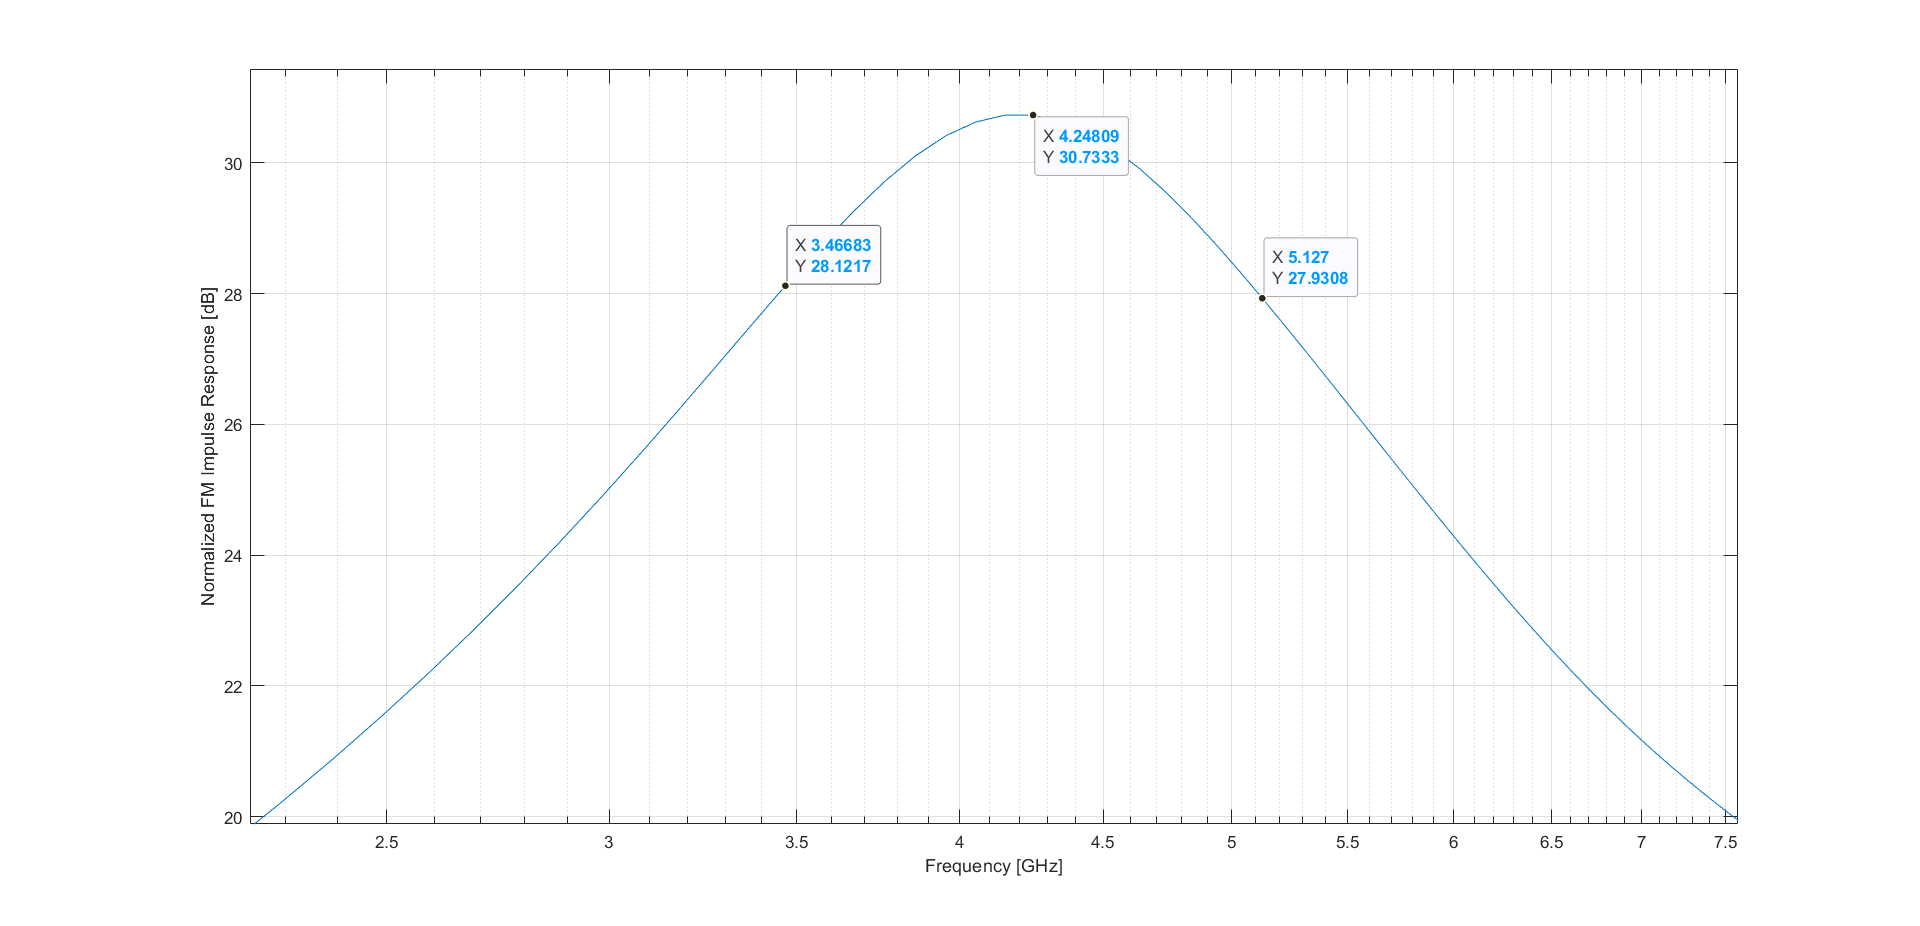
\includegraphics[width=\textwidth]{lab3/Images/prob2/FM_6.png}
        \caption{Risposta FM del laser con $I_b = 6 I_{\text{th}}$}
        \label{fig:FM_6}
    \end{subfigure}
    \hfill
    \begin{subfigure}[b]{0.49\textwidth}
        \centering
        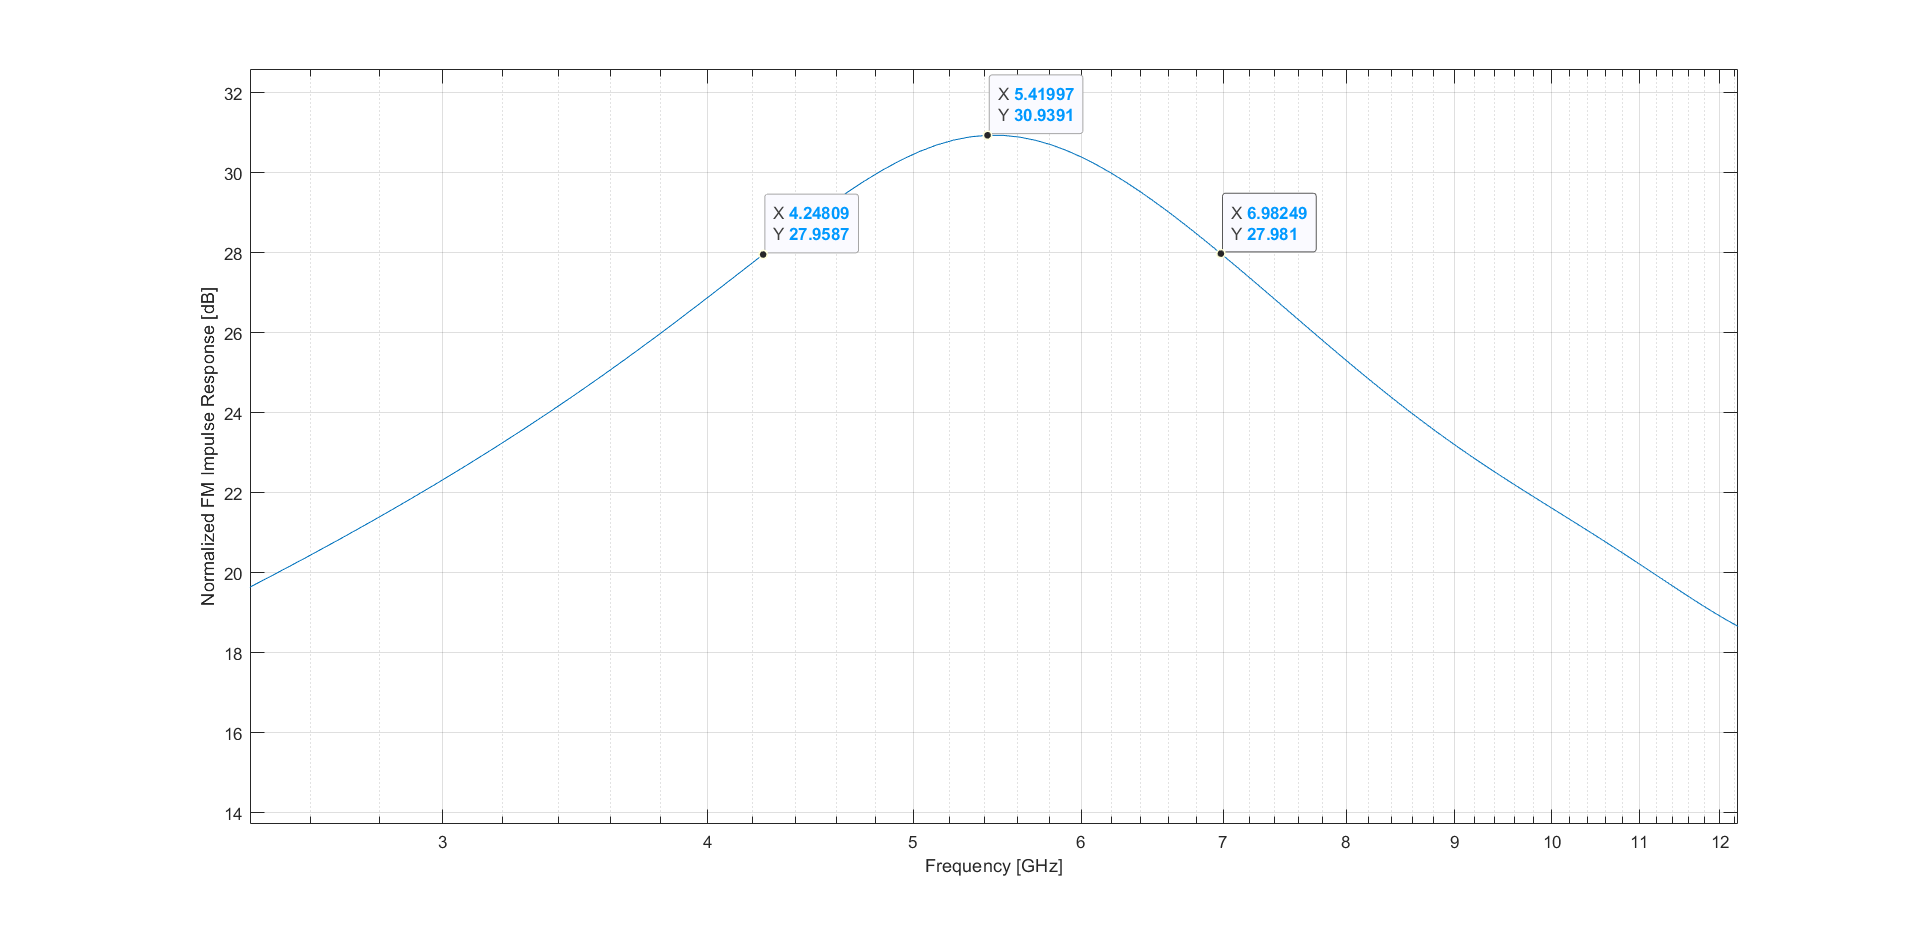
\includegraphics[width=\textwidth]{lab3/Images/prob2/FM_10.png}
        \caption{Risposta FM del laser con $I_b = 10 I_{\text{th}}$}
        \label{fig:FM_10}
    \end{subfigure}
    \caption{Risposta FM del laser con correnti di polarizzazione $I_b = 6 I_{\text{th}}$ e $I_b = 10 I_{\text{th}}$}
    \label{fig:FM_b3_b4}
\end{figure}

\noindent Per la modulazione in frequenza, invece, l'andamento è molto simile a quello dei portatori e proporzionale al LEF $\alpha_H$ che nella simulazione è pari a 1.
In questo caso i valori di banda sono misurati a -3 dB dalla frequenza di picco. I valori di corrente di bias sono i medesimi utilizzati per la risposta IM,
così da poter effettuare un confronto diretto tra i due tipi di modulazione e le rispettive occupazioni spettrali. I risultati sono riportati in Tabella \ref{tab:bandaFM_3dB}.

\begin{table}[!h]
    \centering
    \begin{tabular}{c c}
        \hline
        \textbf{Corrente di bias ($I_{\text{bias}}$)} & \textbf{Banda FM a $-3\text{ dB}$ ($f_{-3\text{dB,peak}}$)} \\
        \hline
        $1.05 \, I_{\text{th}}$ & $680  \text{ MHz}$ \\
        $2.0 \, I_{\text{th}}$  & $2.15 \text{ GHz}$ \\
        $6.0 \, I_{\text{th}}$  & $5.15 \text{ GHz}$ \\
        $10.0 \, I_{\text{th}}$ & $6.98 \text{ GHz}$ \\
        \hline
    \end{tabular}
    \caption{Frequenza a $-3\text{ dB}$ rispetto al picco FM al variare della corrente di polarizzazione}
    \label{tab:bandaFM_3dB}
\end{table}

\noindent Per poter confrontare al meglio le bande delle due tipologie di modulazione, si propone la seguente tabella riassuntiva \ref{tab:confronto_AM_FM}.

\begin{table}[!h]
    \centering
    \begin{tabular}{|c|c|c|}
        \hline
        \textbf{Corrente di bias ($I_{\text{bias}}$)} & \textbf{Banda AM ($f_{-3\text{dB}}$)} & \textbf{Banda FM ($f_{-3\text{dB,peak}}$)} \\ \hline \hline
        $1.05 \, I_{\text{th}}$ & $680 \text{ MHz}$ & $680 \text{ MHz}$ \\ \hline
        $2.0 \, I_{\text{th}}$  & $2.90 \text{ GHz}$ & $2.15 \text{ GHz}$ \\ \hline
        $6.0 \, I_{\text{th}}$  & $6.20 \text{ GHz}$ & $5.15 \text{ GHz}$ \\ \hline
        $10.0 \, I_{\text{th}}$ & $7.65 \text{ GHz}$ & $6.98 \text{ GHz}$ \\  \hline
    \end{tabular}
    \caption{Confronto delle bande di modulazione AM e FM a $-3\text{ dB}$ al variare della corrente di polarizzazione.}
    \label{tab:confronto_AM_FM}
\end{table}

\noindent Dai risultati emerge come la modulazione di frequenza presenti una banda leggermente più ristretta rispetto a quella di intensità, pur seguendo il medesimo trend
di crescita all'aumentare della corrente di polarizzazione.

\noindent\\ Per valutare il limite teorico massimo della banda di modulazione ($f_{-3\text{dB, max}}$), occorre distinguere tra il caso ideale privo di compressione del
guadagno ($\epsilon = 0$, ossia il caso appena analizzato) e il caso reale ($\epsilon \neq 0$).

\paragraph{Caso ideale ($\epsilon = 0$):} 
La banda massima teorica è limitata unicamente dal tempo di vita dei fotoni in cavità $\tau_p$:

\begin{equation}
f_{-3\text{dB, ideale}} = \frac{\sqrt{2}}{\tau_p} \cdot \frac{1}{2\pi}
\end{equation}

\noindent dove:
\[ 
\tau_p = \frac{1}{v_g (\alpha_i + \alpha_m)}
\]

\noindent\\ con $\alpha_i$ che rappresenta le perdite intrinseche del materiale (assorbimento) e $\alpha_m$ le perdite agli specchi. Calcolando il tempo di vita dei fotoni 
con i valori introdotti in precedenza, si trova che $\tau_p \approx 6.83\text{ ps}$. Di conseguenza si ottiene:
\begin{equation}
f_{-3\text{dB, ideale}} \approx \frac{\sqrt{2}}{2\pi \cdot 6.83\text{ ps}} \approx 32.96\text{ GHz}
\end{equation}

\noindent Si osserva un significativo divario tra la banda massima misurata a $10 \, I_{\text{th}}$ ($7.65\text{ GHz}$) e il limite teorico asintotico del sistema.
Tale discrepanza è dovuta al fatto che il valore teorico rappresenta un asintoto ideale valido per densità di fotoni tendenti all'infinito ($I_{\text{bias}} \to \infty$). 

\noindent\\ Aumentando ulteriormente la corrente di polarizzazione nel modello ideale, in linea teorica la frequenza di risonanza
$f_r \propto \sqrt{I_{\text{bias}} - I_{\text{th}}}$ continuerebbe a crescere, permettendo di incrementare la frequenza di taglio. In realtà, nei dispositivi reali questo
incremento è fortemente limitato da molteplici effetti, tra cui il fattore di saturazione del guadagno ($\epsilon \neq 0$) che sarà discusso nel paragrafo successivo.

\noindent\\
\paragraph{Caso reale ($\epsilon \neq 0$):} 
La presenza del fattore di compressione del guadagno $\epsilon = 0.5 \cdot 10^{-16} \text{ cm}^3$ introduce una saturazione che riduce la banda massima raggiungibile secondo la relazione:
\begin{equation}
f_{-3\text{dB, reale}} = f_{-3\text{dB, ideale}} \cdot \left(1 + \frac{\Gamma g_{\text{th}} \epsilon}{a_0}\right)^{-1}
\end{equation}
dove $\Gamma g_{\text{th}} = \alpha_i + \alpha_m$ rappresenta le perdite totali di cavità alla soglia e $a_0$ il guadagno differenziale.

\noindent\\ Sostituendo i parametri del dispositivo, si ottiene una drastica riduzione della banda massima effettiva:
\begin{equation}
f_{-3\text{dB, reale}} \approx 32.96\text{ GHz} \cdot \left(1 + \frac{(6+14.5) \cdot 0.5 \cdot 10^{-16}}{1.5 \cdot 10^{-16}}\right)^{-1} \approx 4.21\text{ GHz}
\end{equation}

\noindent\\\\ Per verificare sperimentalmente tramite simulazione l'effetto del fattore di compressione del guadagno, vengono di seguito riportati i grafici delle risposte
in frequenza IM (Figura \ref{fig:eps1_IM_10}) e FM (Figura \ref{fig:eps1_FM_10}) ottenuti impostando $\epsilon = 0.5 \cdot 10^{-16} \text{ cm}^3$ e la corrente di bias
maggiore analizzata in precedenza, ovvero $I_b = 10 I_{\text{th}}$.

\newpage

\begin{figure}[!h]
 \centering
 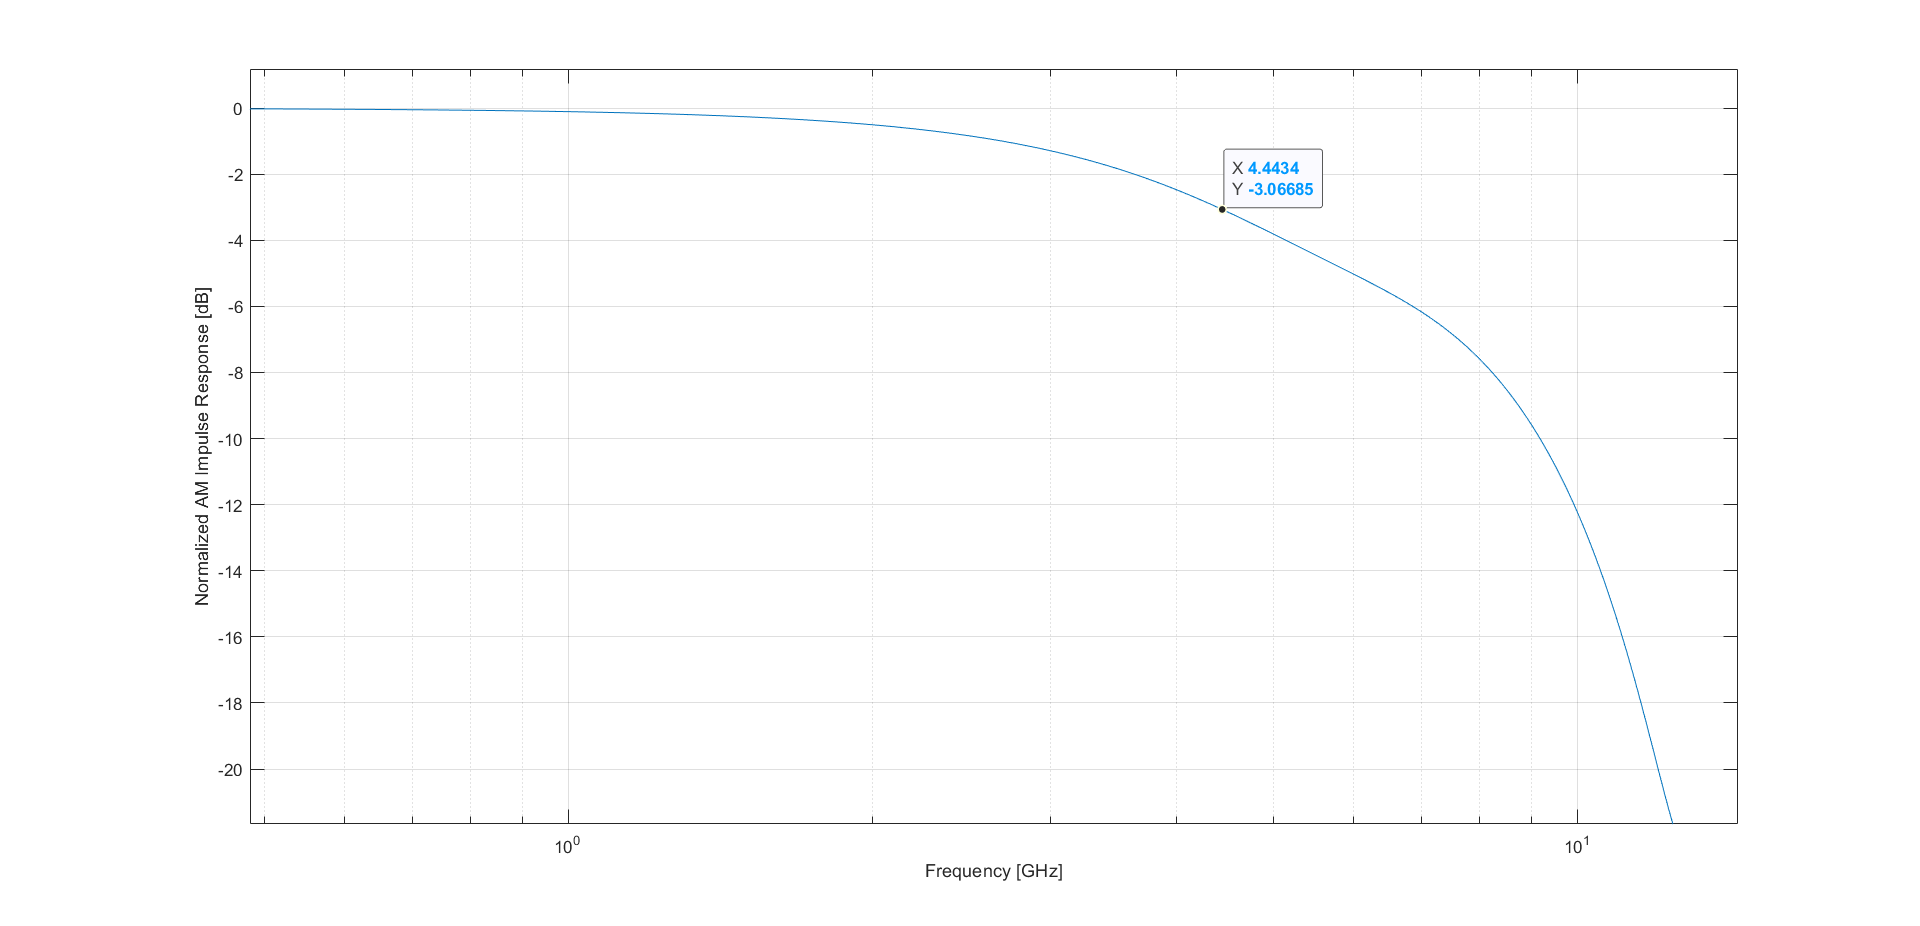
\includegraphics[width=15cm]{lab3/Images/prob2/eps1/eps1_IM_10.png}
  \caption{Risposta AM del laser con $I_b = 10 I_{\text{th}}$ e $\epsilon = 0.5 \cdot 10^{-16} \text{ cm}^3$}
  \label{fig:eps1_IM_10}
\end{figure}

\begin{figure}[!h]
 \centering
 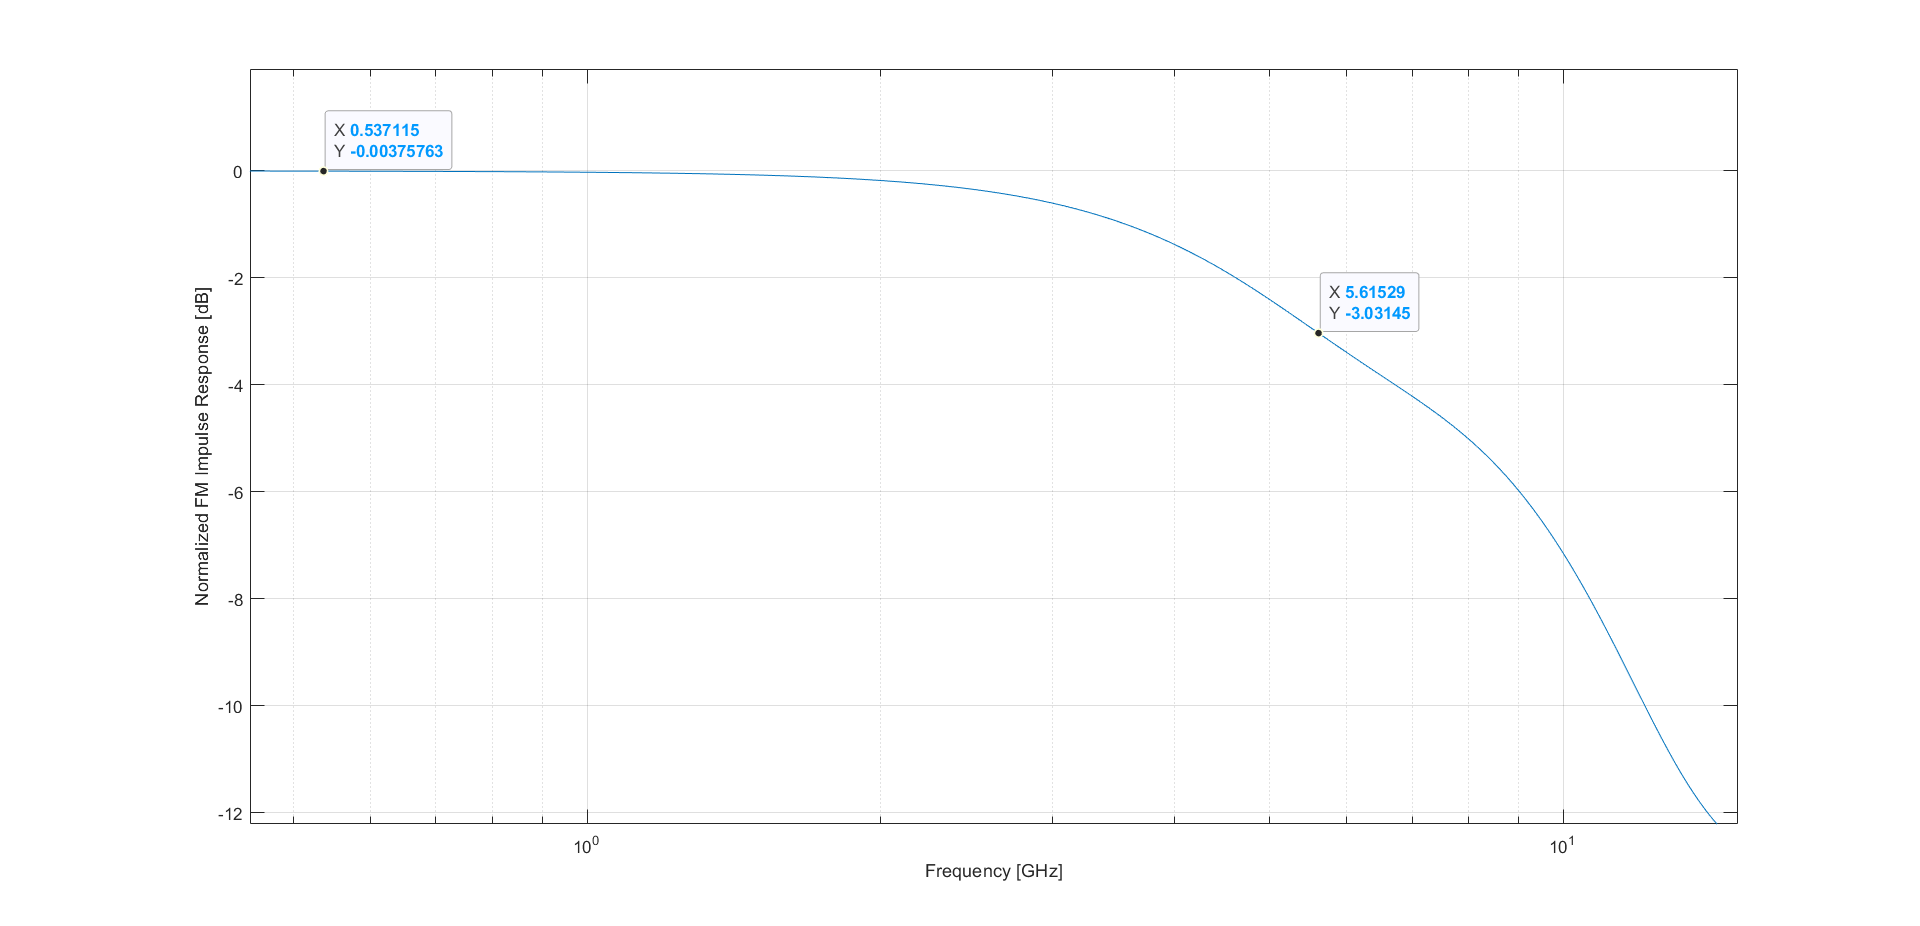
\includegraphics[width=15cm]{lab3/Images/prob2/eps1/eps1_FM_10.png}
  \caption{Risposta FM del laser con $I_b = 10 I_{\text{th}}$ e $\epsilon = 0.5 \cdot 10^{-16} \text{ cm}^3$}
  \label{fig:eps1_FM_10}
\end{figure}

\noindent Dalle Figure riportate sopra, risulta molto evidente e marcato l'effetto del fattore di compressione del guadagno, che riduce drasticamente la banda di modulazione
a $-3\text{ dB}$ per la risposta IM, che adesso è molto prossima al limite teorico calcolato. I risultati ottenuti sono riassunti nella seguente tabella \ref{tab:eps1_bandaAM_FM_3dB}.

\begin{table}[!h]
    \centering
    \begin{tabular}{|c|c|c|}
        \hline
        \textbf{Corrente di bias ($I_{\text{bias}}$)} & \textbf{Banda AM ($f_{-3\text{dB}}$)} & \textbf{Banda FM ($f_{-3\text{dB,peak}}$)} \\ \hline \hline
        $1.05 \, I_{\text{th}}$ & $670 \text{ MHz}$ & $670 \text{ MHz}$ \\ \hline
        $2.0 \, I_{\text{th}}$  & $2.59 \text{ GHz}$ & $2.53 \text{ GHz}$ \\ \hline
        $6.0 \, I_{\text{th}}$  & $3.76 \text{ GHz}$ & $5.05 \text{ GHz}$ \\ \hline
        $10.0 \, I_{\text{th}}$ & $4.44 \text{ GHz}$ & $5.62 \text{ GHz}$ \\  \hline
    \end{tabular}
    \caption{Confronto delle bande di modulazione AM e FM a $-3\text{ dB}$ al variare della corrente di polarizzazione.}
    \label{tab:eps1_bandaAM_FM_3dB}
\end{table}

\noindent Occorre evidenziare che il limite teorico di banda massima $f_{-3\text{dB, reale}} \approx 4.21\text{ GHz}$ (e la relativa trattazione del \textit{damping limit}) è
stato ricavato analiticamente a partire dalla risposta in intensità (IM/AM). Di conseguenza, i valori di banda FM ricavati dalle simulazioni ($5.62\text{ GHz}$ a $10 I_{\text{th}}$) superano il limite teorico calcolato per l'AM, riflettendo la
diversa dinamica di accoppiamento fase-ampiezza del campo ottico.
\noindent Un ulteriore aspetto fondamentale che emerge dal confronto delle risposte FM con fattore di compressione del guadagno ($\epsilon = 0.5 \cdot 10^{-16}\text{ cm}^3$)
riguarda la progressiva scomparsa del picco di risonanza all'aumentare della corrente di polarizzazione. 

\noindent\\ Mentre nel caso ideale ($\epsilon = 0$) l'aumento di $I_b$ sposta la frequenza di risonanza $f_r$ verso destra mantenendo un picco pronunciato, l'introduzione di
$\epsilon \neq 0$ incrementa drasticamente il fattore di smorzamento (\textit{damping factor}) $\gamma$. Ad alte correnti di polarizzazione ($I_b = 6 I_{\text{th}}$ e
$10 I_{\text{th}}$), l'elevata densità di fotoni in cavità rende il termine di smorzamento sovrastante rispetto alla risonanza, provocando il completo appiattimento
del picco di risonanza (\textit{overdamped response}) e convertendo la risposta FM in un profilo passa-basso a decadimento dolce.


\newpage
\section{Modulazione diretta NRZ con PRBS}
Di seguito sono riportati i grafici ottenuti per la simulazione della modulazione diretta NRZ del laser con una sequenza PRBS. I parametri di corrente sono:
\begin{itemize}
    \item Corrente minima: $I_{min} = 0.5 I_{\text{th}}$
    \item Corrente massima: $I_{max} = 2 I_{\text{th}}$
    \item Bit-rate: $B_r = 2.5 \, \text{Gb/s}$ 
\end{itemize}

\noindent I risultati dell'analisi dinamica sono riportati in Figura \ref{fig:PRBS_1}

\begin{figure}[!h]
 \centering
 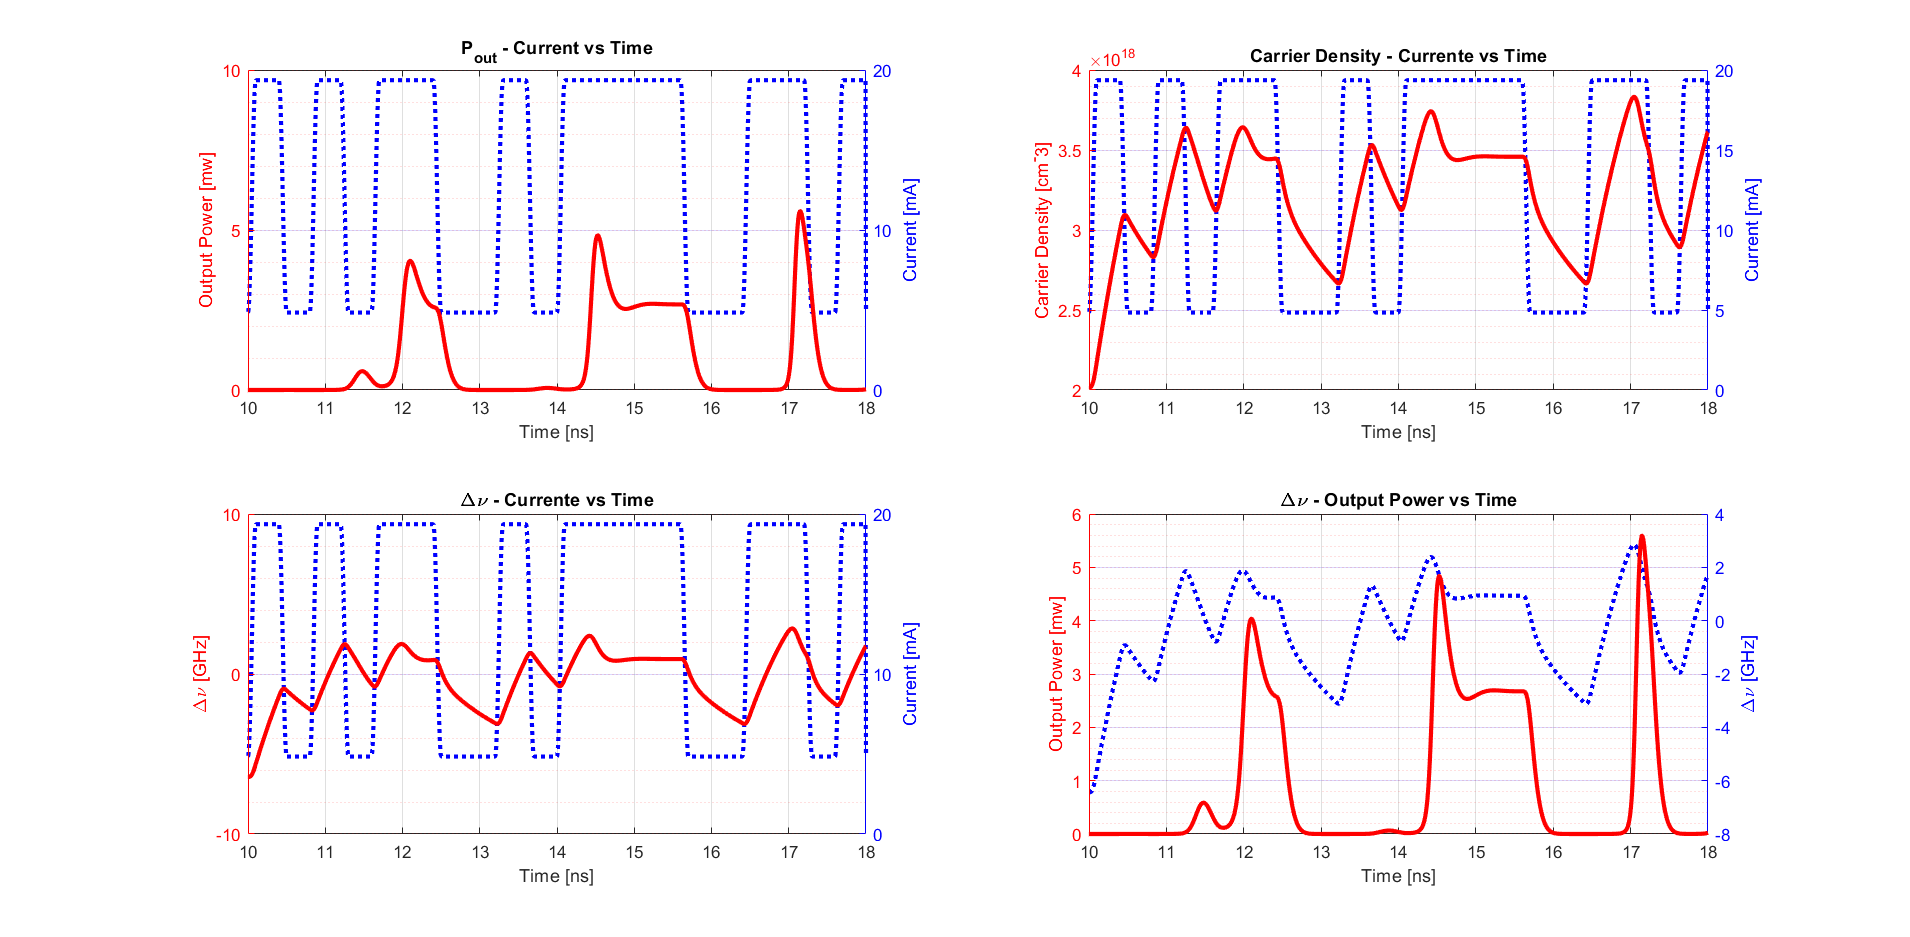
\includegraphics[width=15cm]{lab3/Images/prob3/PRBS_1.png}
  \caption{Simulazione PRBS con $I_{min} = 0.5 I_{\text{th}}$, $I_{max} = 2 I_{\text{th}}$ e $B_r = 2.5 \, \text{Gb/s}$}
  \label{fig:PRBS_1}
\end{figure}

I quattro plot della Figura precedente mostrano:
\begin{itemize}
    \item \textbf{Potenza in uscita vs Tempo}: La potenza segue l'andamento del segnale di corrente, ma con una risposta non istantanea dovuta alla dinamica del laser.
    \item \textbf{Densità dei portatori vs Tempo}: La densità dei portatori segue l'andamento del segnale di corrente, con oscillazioni dovute ai tempi di ricombinazione e
    di iniezione dei portatori.
    \item \textbf{Frequency chirp vs Tempo}: La frequenza del laser varia in funzione del tempo, mostrando oscillazioni che riflettono la variazione della corrente
    di iniezione.
    \item \textbf{Frequency chirp vs Potenza in uscita}: La relazione tra potenza e variazione della frequenza mostra il comportamento del chirp indotto dalla modulazione
    diretta.
\end{itemize}

\subsubsection{Confronto tra segnale di corrente e segnale di potenza}
\noindent Dal grafico Potenza vs Tempo emerge chiaramente come la potenza in uscita segua l'andamento del segnale di corrente, evidenziando tuttavia un ritardo temporale
dovuto alla risposta dinamica del laser. Le transizioni tra i livelli alti e bassi di corrente non avvengono in modo istantaneo, ma mostrano fenomeni di overshoot e
undershoot. Inoltre, nei livelli bassi la potenza non riproduce fedelmente il profilo della corrente a causa dell'effetto della soglia del laser.

\noindent\\ Questo comportamento trova spiegazione nei tempi di ricombinazione, poiché la densità dei portatori impiega un tempo finito per raggiungere lo stato stazionario,
e nell'accumulo di carica nella cavità, che ritarda la risposta dinamica in quanto i fotoni richiedono tempo prima di accumularsi e innescare l'emissione stimolata.
Inoltre, a correnti più elevate subentrano gli effetti di compressione del guadagno, il quale si riduce a causa della saturazione della popolazione dei portatori.

\noindent\\ Risulta quindi evidente come modulare il laser con un ampio segnale portandolo al di sotto della condizione di soglia (ossia con $I_{\text{min}} < I_{\text{th}}$)
comprometta il corretto funzionamento del dispositivo, anche qualora la frequenza del segnale modulante ricada teoricamente all'interno della banda passante del laser.
Di conseguenza, nel caso di una modulazione ad ampio segnale, risulta decisamente più conveniente mantenere il laser costantemente acceso, imponendo una corrente minima
che sia strettamente superiore a quella di soglia ($I_{\text{min}} > I_{\text{th}}$).

\subsection{Simulazione PRBS sopra-soglia}
In questa sottosezione vengono riportati i risultati della simulazione della modulazione diretta NRZ del laser con una sequenza PRBS, dove la corrente di iniezione è mantenuta
sempre al di sopra della soglia:
\begin{itemize}
    \item Corrente minima: $I_{min} = 1.5 I_{\text{th}}$
    \item Corrente massima: $I_{max} = 4 I_{\text{th}}$
    \item Bit-rate: $B_r = 2.5 \, \text{Gb/s}$ 
\end{itemize}

\noindent I risultati della simulazione sono mostrati nella seguente Figura:

\begin{figure}[!h]
 \centering
 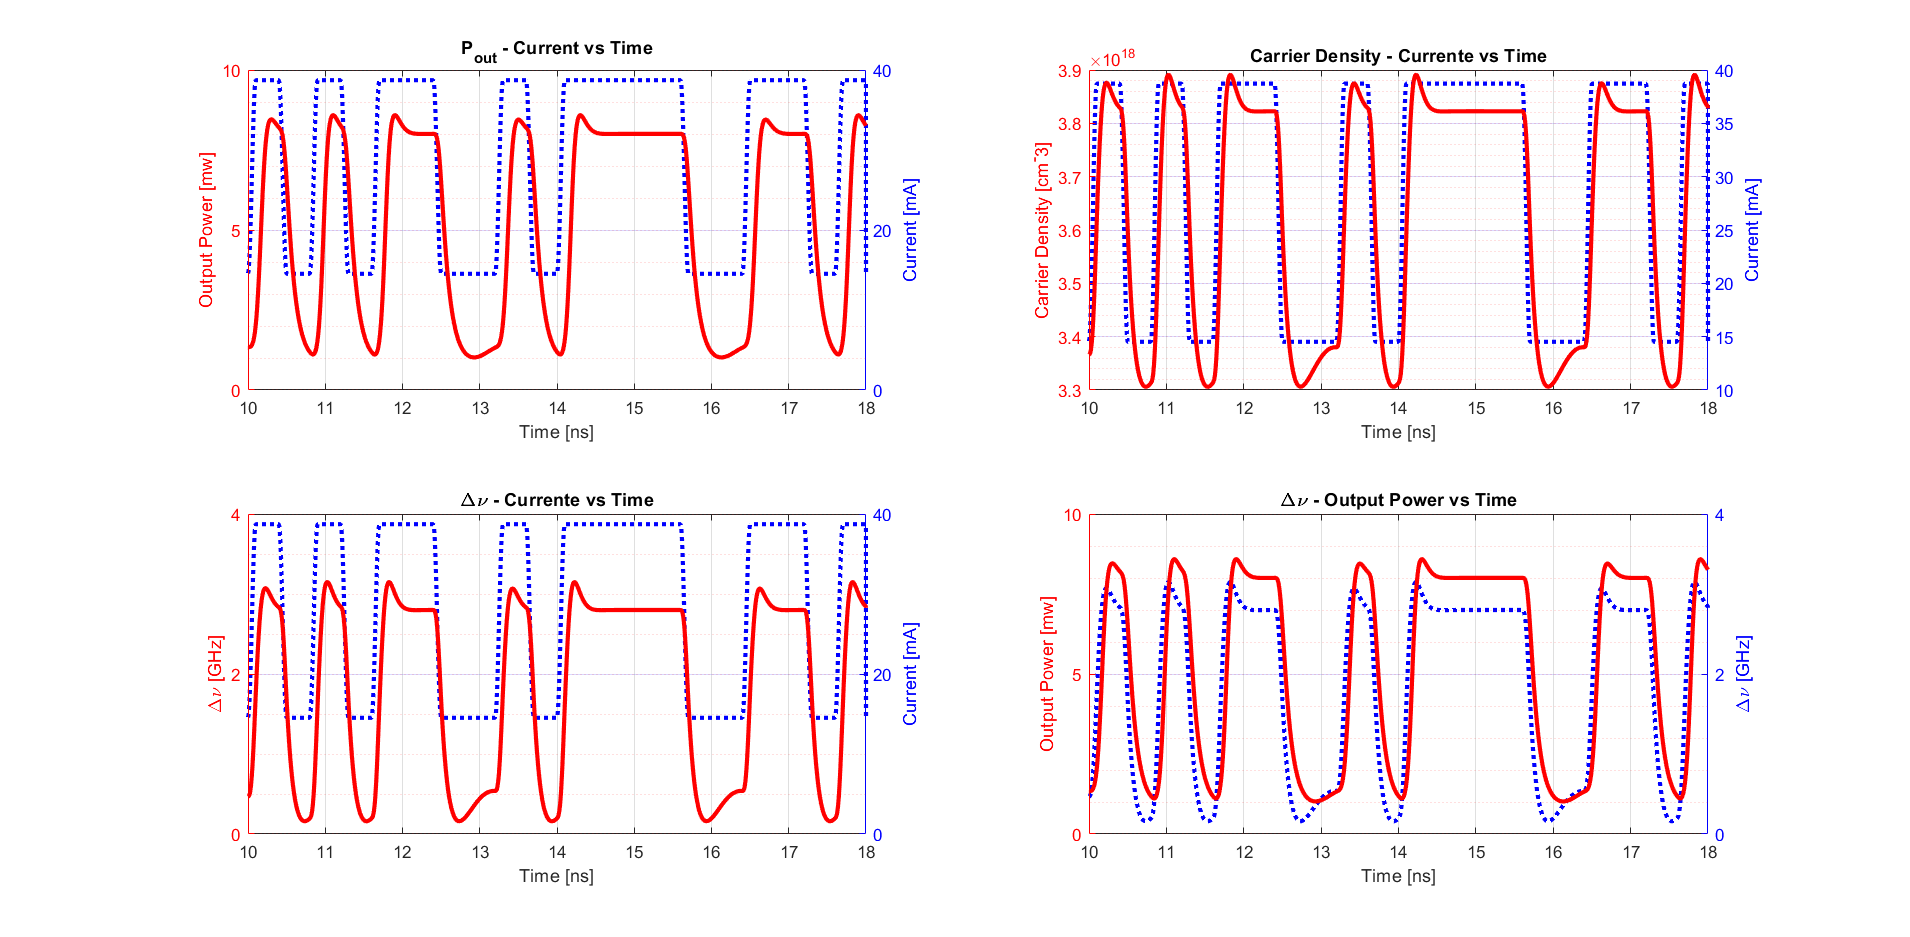
\includegraphics[width=15cm]{lab3/Images/prob3/PRBS_2.png}
  \caption{Simulazione PRBS con $I_{min} = 1.5 I_{\text{th}}$, $I_{max} = 4 I_{\text{th}}$ e $B_r = 2.5 \, \text{Gb/s}$}
  \label{fig:PRBS_2}
\end{figure}

\noindent Dal confronto tra il segnale di corrente e la potenza in uscita (\ref{fig:PRBS_2}), si osserva che quest'ultima segue in modo molto più fedele l'andamento della corrente
rispetto a quanto riscontrato nella simulazione precedente (\ref{fig:PRBS_1}). L'assenza di tempi morti significativi è riconducibile al fatto che il laser opera costantemente
in regime di emissione stimolata. Di conseguenza, il comportamento dinamico del dispositivo risulta notevolmente più lineare e prevedibile rispetto al caso in cui la
corrente scende al di sotto della soglia.

\subsubsection{Differenze rispetto alla simulazione precedente e conclusioni}
Dal confronto con il caso precedente, in cui la corrente variava tra $0.5 I_{\text{th}}$ e $2 I_{\text{th}}$, emergono sostanziali differenze.
Operando costantemente al di sopra della soglia, l'accensione e lo spegnimento avvengono in tempi decisamente più rapidi, e la potenza in uscita riproduce con maggiore
fedeltà il segnale di corrente, presentando oscillazioni transitorie nettamente ridotte. Inoltre, l'assenza di attraversamenti della soglia limita le rapide fluttuazioni
della densità dei portatori, rendendo il \textit{frequency chirp} sensibilmente meno pronunciato.

\noindent\\ In conclusione, mantenere la corrente di modulazione sempre al di sopra della soglia migliora in modo significativo la risposta dinamica del laser, garantendo
un comportamento più lineare e prevedibile e riducendo le distorsioni del segnale ottico. Sebbene questa modalità operativa comporti uno svantaggio in termini di maggior
consumo energetico e dissipazione termica nel dispositivo, essa si rivela fondamentale nelle comunicazioni ottiche ad alta velocità, dove una risposta rapida e una ridotta
variabilità di frequenza sono requisiti essenziali per minimizzare la dispersione cromatica e il conseguente degrado del segnale.

\newpage
\section{Modulazione a vari bit-rate e calcolo dell'ER}
La modulazione di tipo NRZ (\textit{Non Return to Zero}) del laser eseguita a diversi bit rate mostra quale può essere il limite di banda e se la comunicazione avviene
in modo corretto. Come spiegato nella sezione precedente, è molto conveniente mantenere il laser sopra soglia per migliorarne la risposta.\\ Di seguito sono riportati
i grafici relativi a potenza in uscita, densità dei portatori e chirp in frequenza:

\begin{figure}[!h]
 \centering
 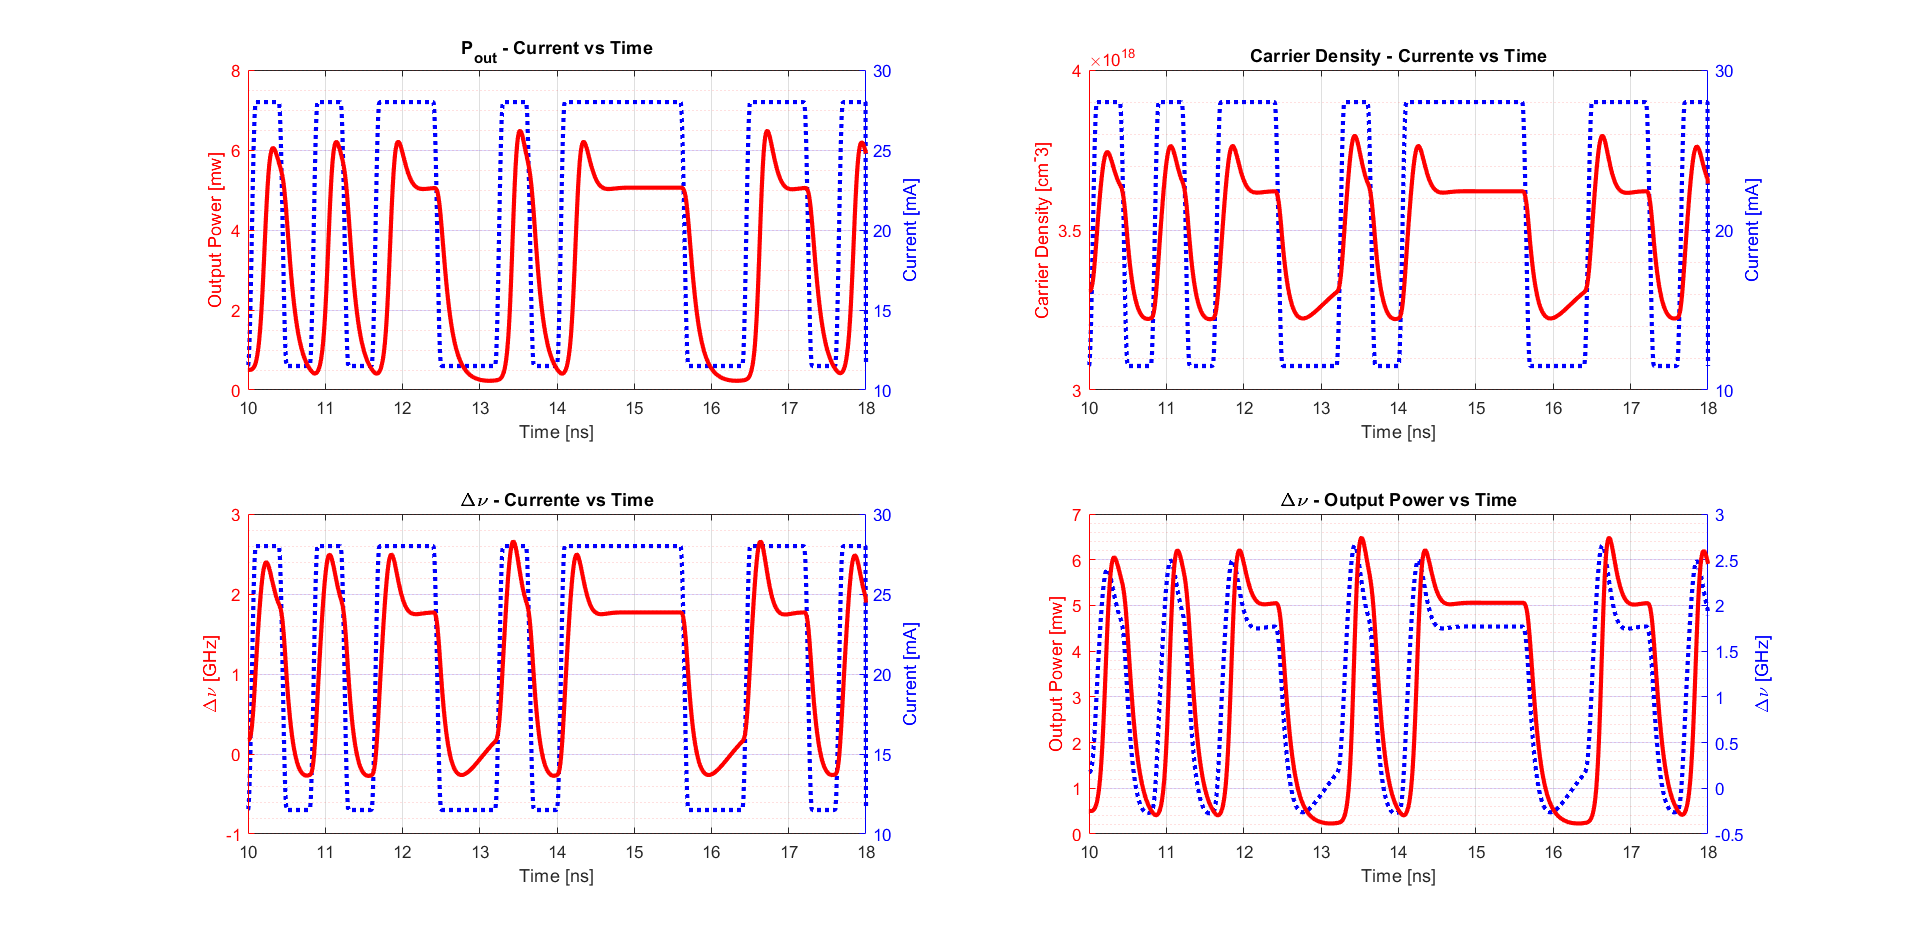
\includegraphics[width=15cm]{lab3/Images/prob4/PRBS_2_5.png}
  \caption{Modulazione NRZ con $B_r = 2.5 \, \text{Gb/s}$}
  \label{fig:PRBS_2_5}
\end{figure}

\noindent Dalla Figura \ref{fig:PRBS_2_5} è possibile identificare un overshoot nella risposta di potenza prima che il segnale ottico si stabilizzi. A questo transitorio di portatori
corrisponde il cosiddetto \textit{Transient Chirp}, legato alla rapida variazione temporale della densità dei portatori ($dN/dt$). Una volta esaurito il transitorio, la
densità dei portatori e la frequenza di emissione si stabilizzano nel regime di \textit{Adiabatic Chirp}.

\noindent\\ Con una modulazione a $2.5\text{ Gbit/s}$, il segnale si mantiene all'interno della banda massima del laser precedentemente valutata. Tuttavia, all'aumentare del bit-rate,
la potenza ottica non riesce più a seguire fedelmente le rapide variazioni della corrente di modulazione a causa della banda limitata del dispositivo; di conseguenza, le
transizioni veloci accentuano gli effetti del chirp e compromettono l'integrità del segnale.

\begin{figure}[!h]
 \centering
 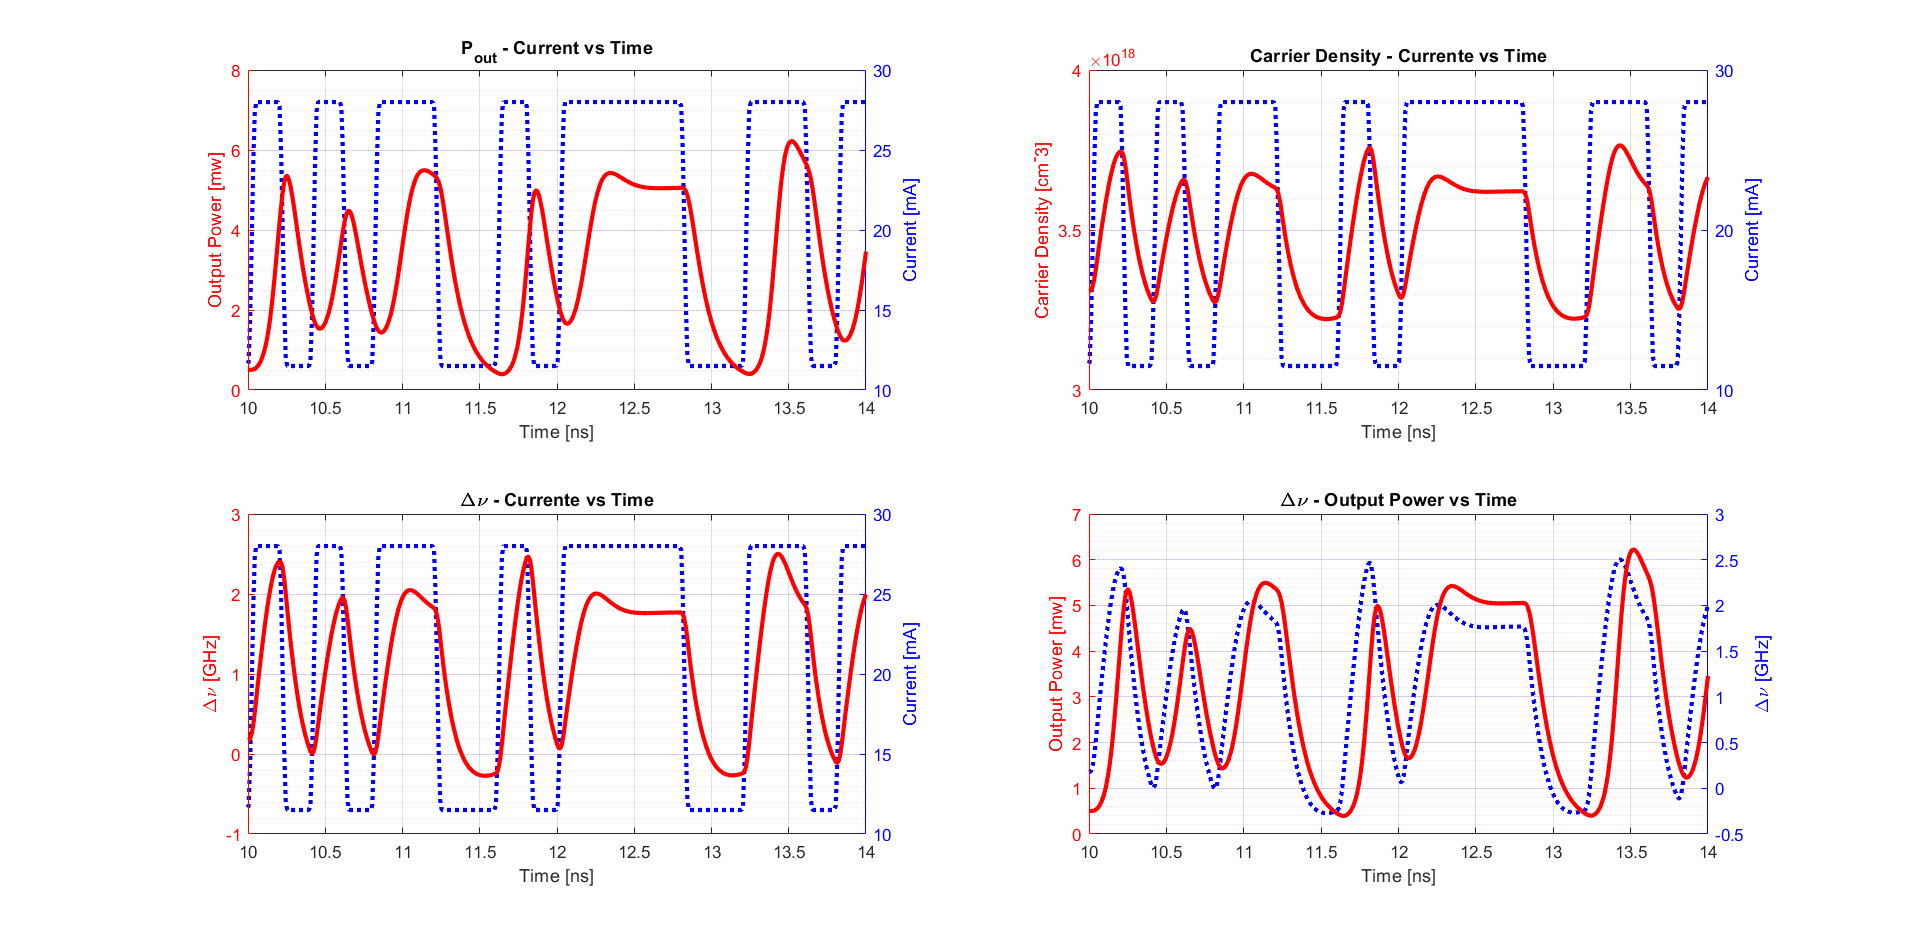
\includegraphics[width=15cm]{lab3/Images/prob4/PRBS_5.png}
  \caption{Modulazione NRZ con $B_r = 5 \, \text{Gb/s}$}
  \label{fig:PRBS_5}
\end{figure}

\newpage

\begin{figure}[!h]
 \centering
 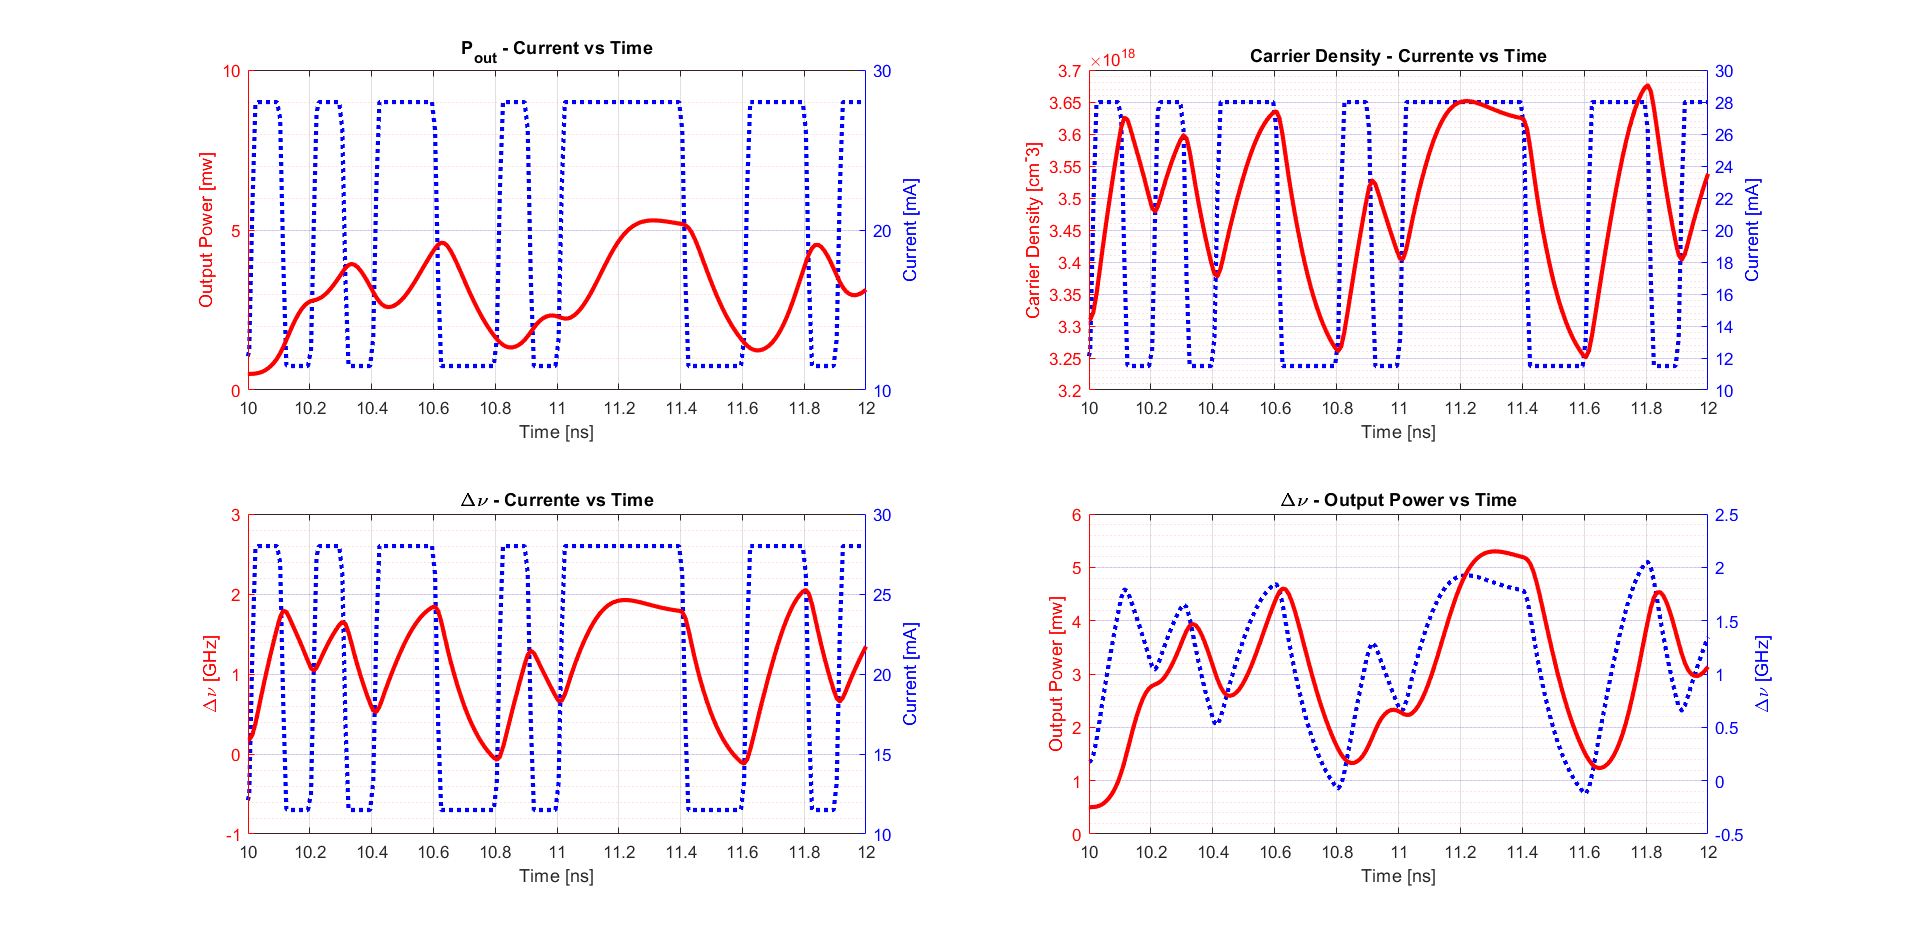
\includegraphics[width=14.3cm]{lab3/Images/prob4/PRBS_10.png}
  \caption{Modulazione NRZ con $B_r = 10 \, \text{Gb/s}$}
  \label{fig:PRBS_10}
\end{figure}

\begin{figure}[!h]
 \centering
 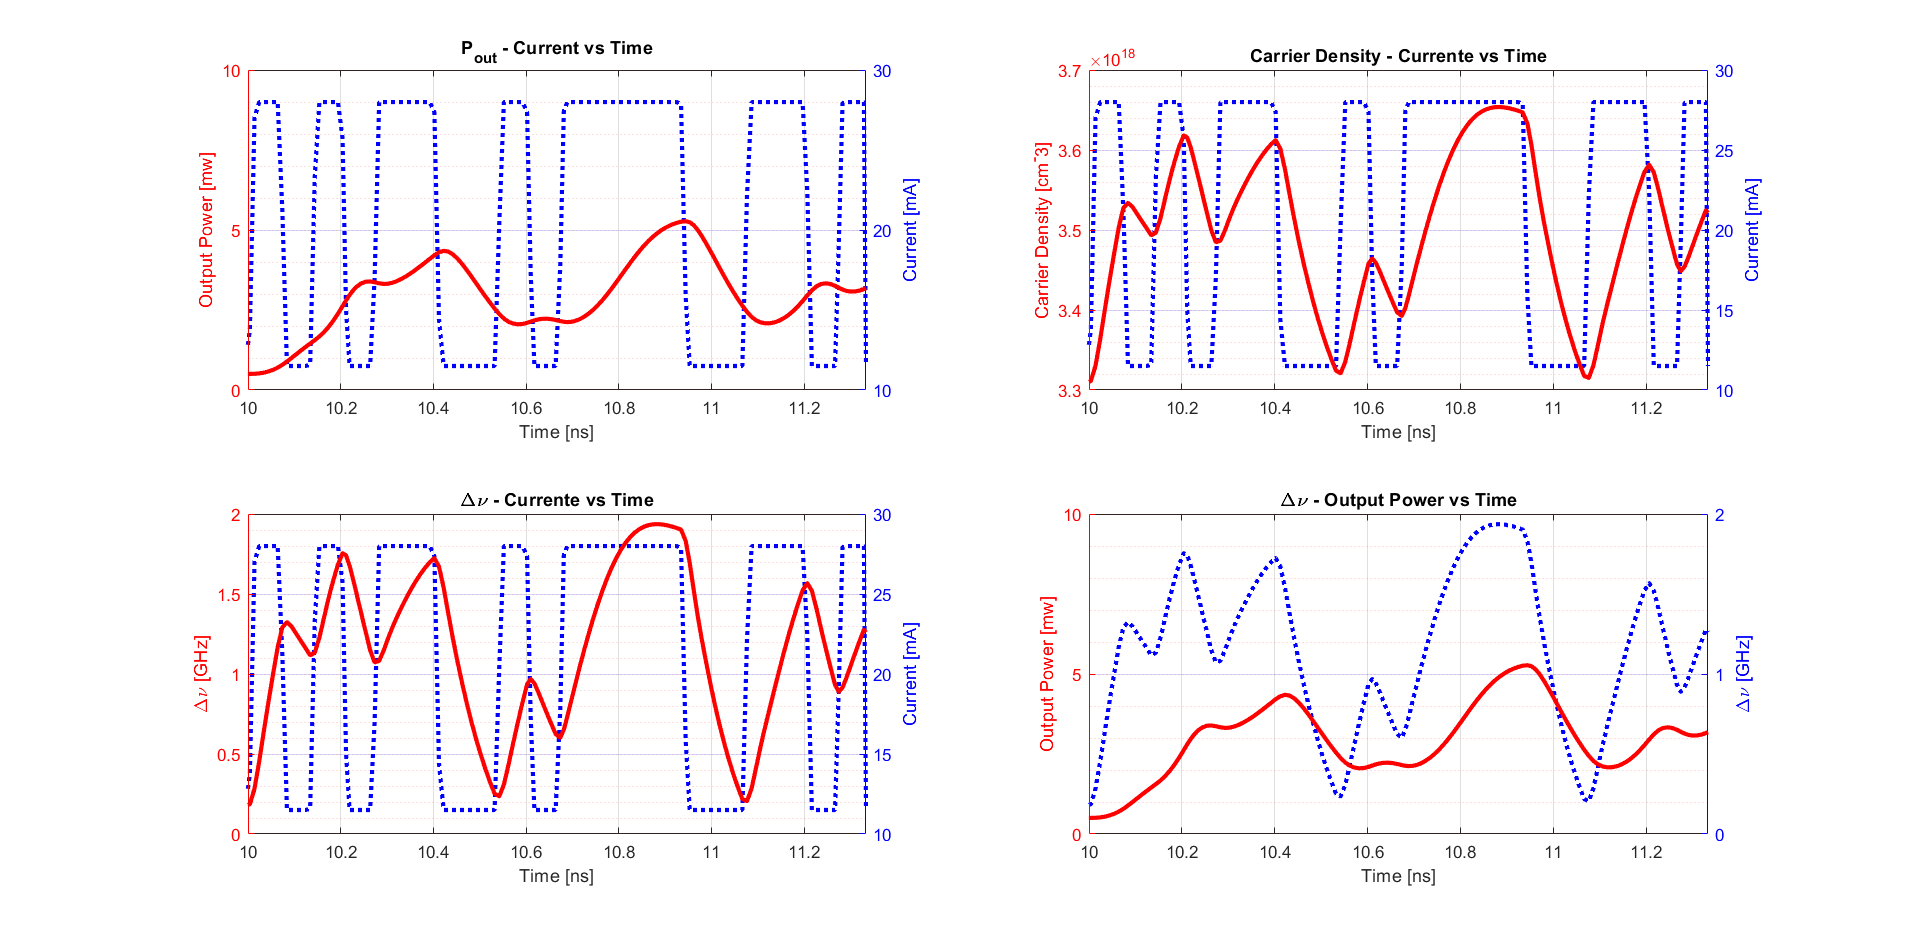
\includegraphics[width=14.3cm]{lab3/Images/prob4/PRBS_15.png}
  \caption{Modulazione NRZ con $B_r = 15 \, \text{Gb/s}$}
  \label{fig:PRBS_15}
\end{figure}

\begin{figure}[!h]
 \centering
 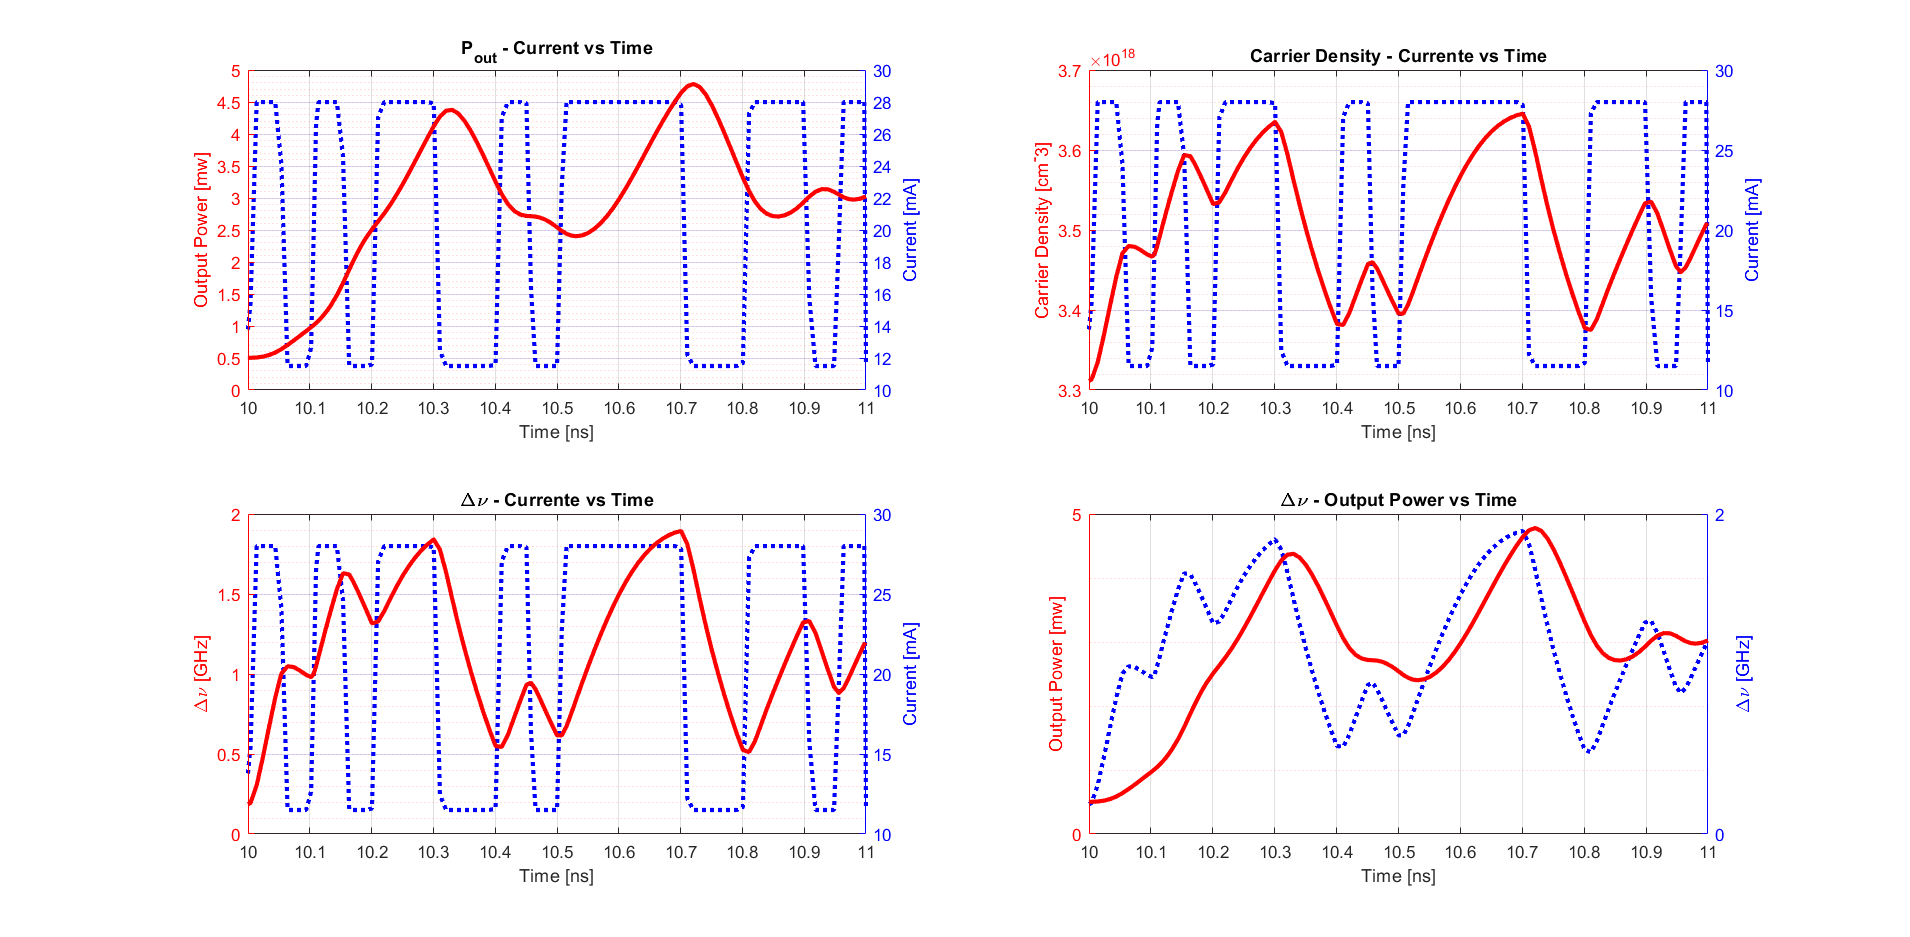
\includegraphics[width=14.3cm]{lab3/Images/prob4/PRBS_20.png}
  \caption{Modulazione NRZ con $B_r = 20 \, \text{Gb/s}$}
  \label{fig:PRBS_20}
\end{figure}

\newpage
\noindent Se la frequenza di modulazione non è troppo elevata, l'integrità del segnale all'uscita dal trasmettitore può essere valutata mediante il diagramma ad occhio
(\textit{Eye Diagram}), che permette di individuare visivamente l'istante ottimale di campionamento in base al raggiungimento del valore a regime dello stato logico.
Tale diagramma consente di stabilire se i due livelli logici risultino ben distinguibili (\textit{occhio aperto}) o se, a causa di una frequenza eccessivamente elevata,
le transizioni si sovrappongano impedendo di mantenere livelli di tensione stabili (\textit{occhio chiuso}).
\noindent Nel seguito sono riportati i diagrammi ad occhio ottenuti per le simulazioni a diversi bit-rate.

\begin{figure}[!h]
  \centering
  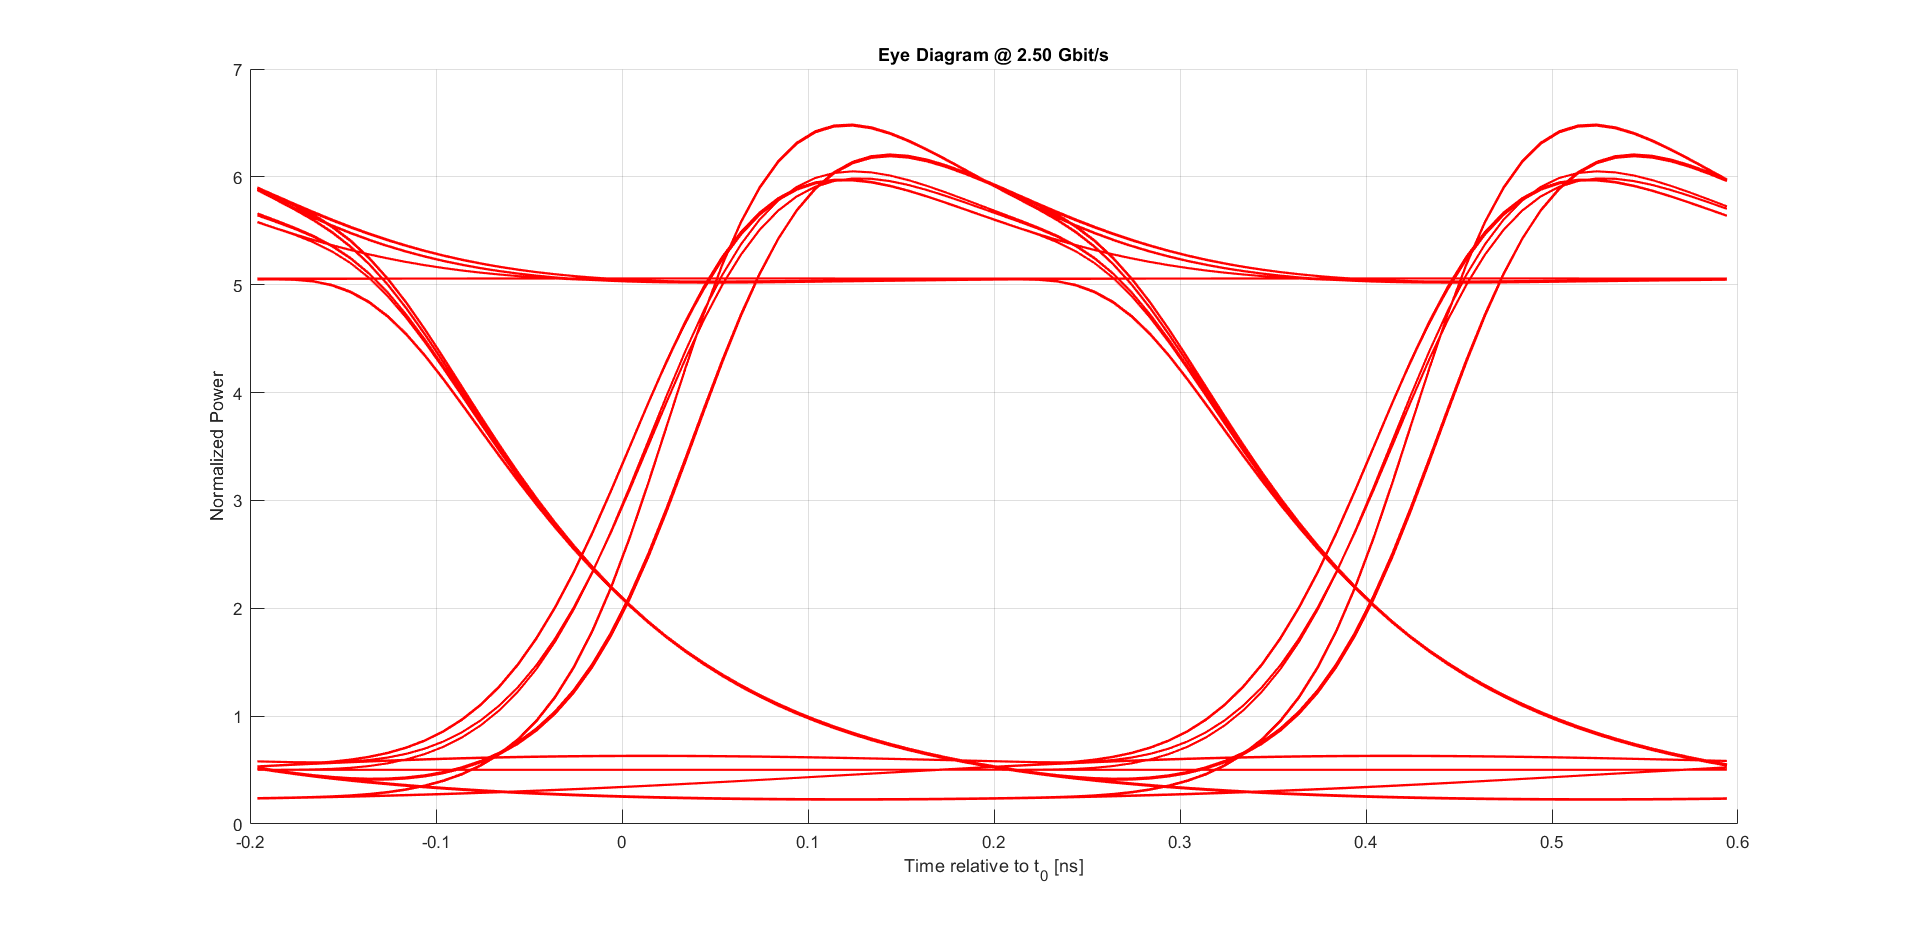
\includegraphics[width=15cm]{lab3/Images/prob4/eye2_5.png}
  \caption{Diagramma ad occhio per un bit-rate di $2.5 \, \text{Gbit/s}$.}
  \label{fig:eye2_5}
\end{figure}

\noindent Dalla Figura \ref{fig:eye2_5}, relativa a un bit-rate di $2.5 \, \text{Gbit/s}$, si osserva un'apertura dell'occhio particolarmente ampia. Questo garantisce un elevato
margine di separazione tra il livello logico alto e quello basso, assicurando una trasmissione compatibile con una corretta discriminazione dei livelli logici.

\begin{figure}[!h]
  \centering
  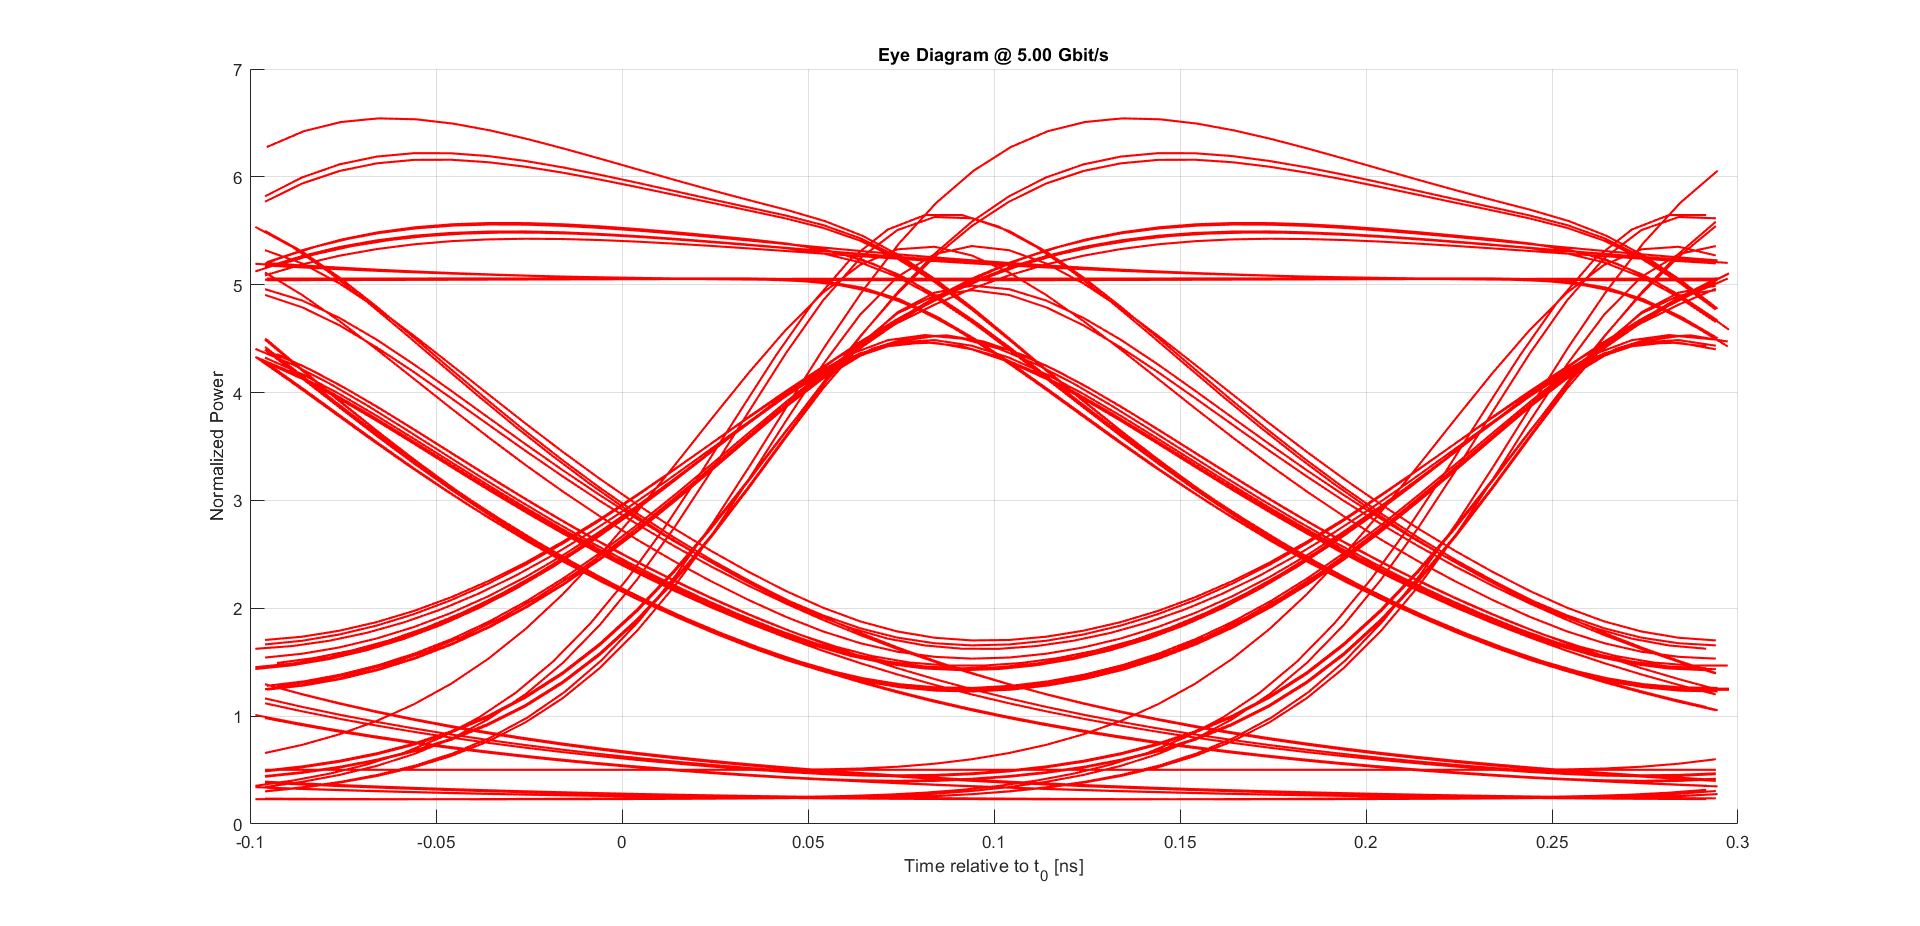
\includegraphics[width=15cm]{lab3/Images/prob4/eye5.png}
  \caption{Diagramma ad occhio per un bit-rate di $5 \, \text{Gbit/s}$.}
  \label{fig:eye5}
\end{figure}

\noindent Aumentando il bit-rate a $5 \, \text{Gbit/s}$ (Figura \ref{fig:eye5}), l'occhio risulta visibilmente più chiuso rispetto al caso precedente, riducendo il
margine di rumore a disposizione. Tuttavia, la separazione tra i livelli logici rimane sufficiente, permettendo ancora
l'impiego del laser a questa frequenza.

\newpage
\begin{figure}[!h]
  \centering
  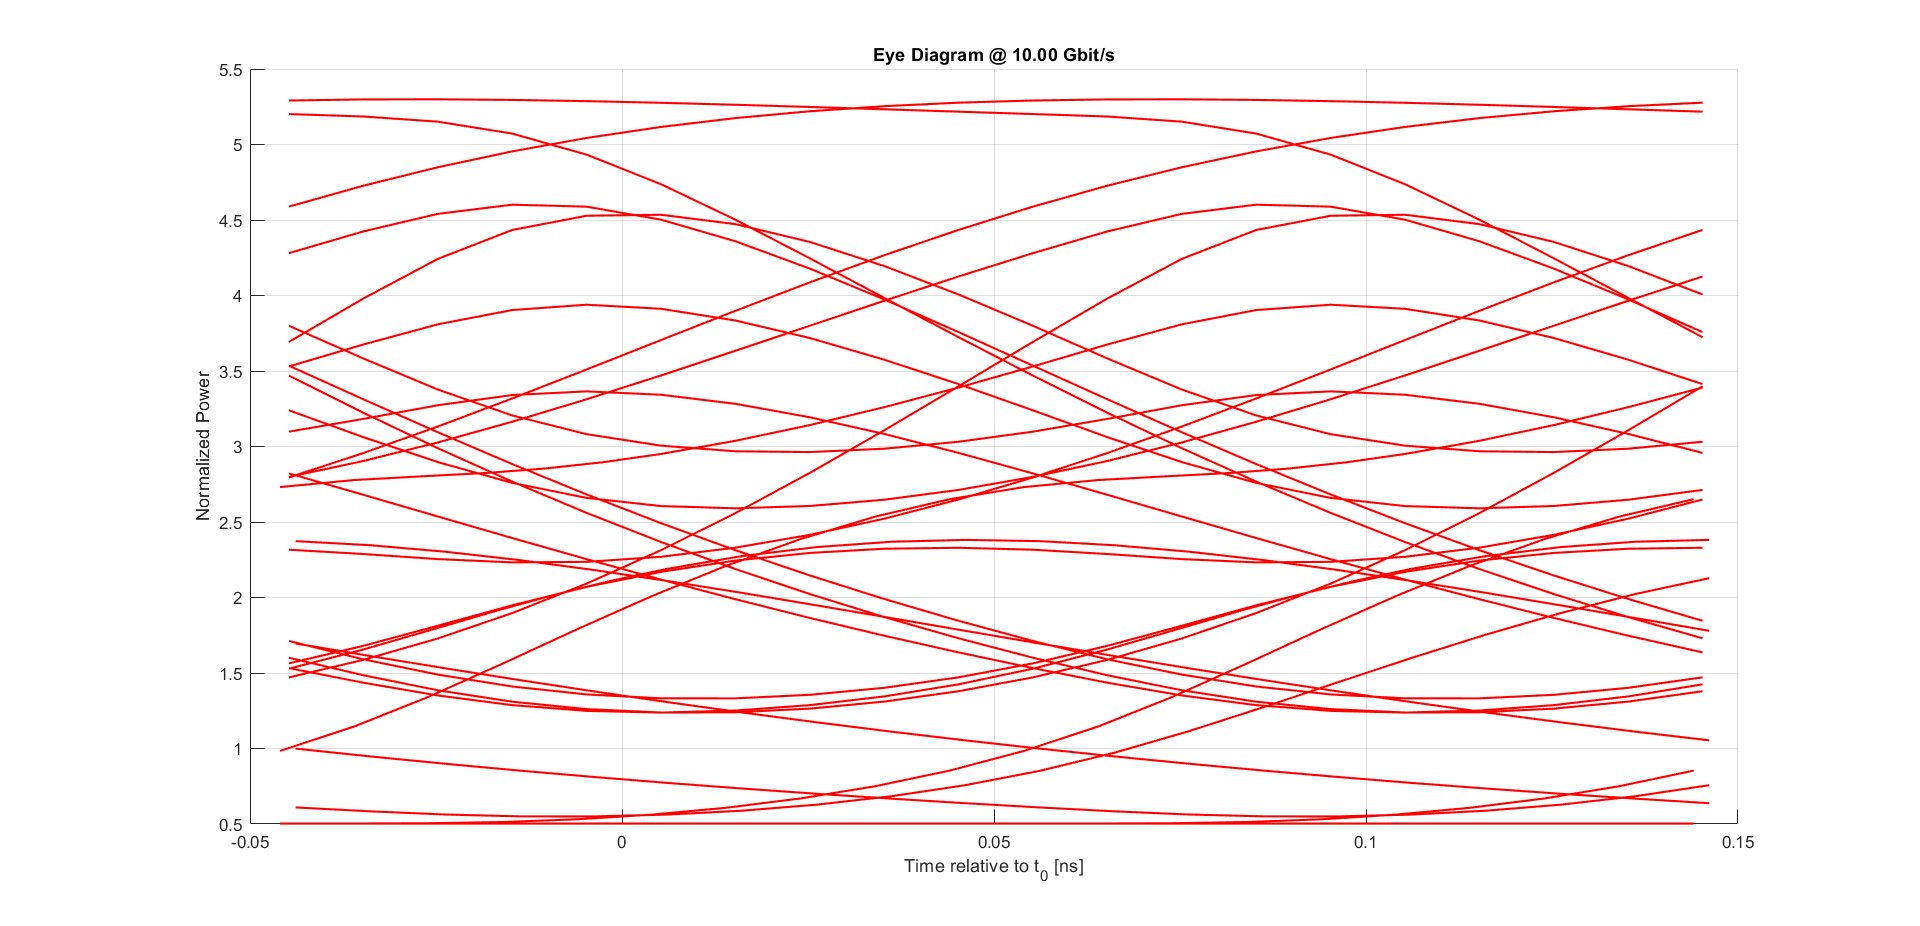
\includegraphics[width=15cm]{lab3/Images/prob4/eye10.png}
  \caption{Diagramma ad occhio per un bit-rate di $10 \, \text{Gbit/s}$.}
  \label{fig:eye10}
\end{figure}

\noindent Infine, portando il bit-rate a $10 \, \text{Gbit/s}$ (Figura \ref{fig:eye10}), il diagramma ad occhio appare quasi completamente chiuso. In queste condizioni, l'elevata
interferenza intersimbolica e il limitato tempo di risposta del laser non consentono più una trasmissione dati affidabile. Per tale motivo, i risultati relativi a bit-rate
superiori non vengono riportati, in quanto le prestazioni del sistema risulterebbero ulteriormente compromesse.